%%%%%%%%%%%%%%%%
%%% DOCUMENT %%%
%%%%%%%%%%%%%%%%
\documentclass[12pt]{article}

%%%%%%%%%%%%%%%%
%%% HEADINGS %%%
%%%%%%%%%%%%%%%%
\pagestyle{headings}

%%%%%%%%%%%%%%%%
%%% PACKAGES %%%
%%%%%%%%%%%%%%%%
\usepackage[english]{babel}
\usepackage{graphicx}
\usepackage{amssymb,amscd}
\usepackage{amsmath}
\usepackage{bbm}
\usepackage{graphics}

%%%%%%%%%%%%%%%%%%%%%%%%%%
%%% PAGE CONFIGURATION %%%
%%%%%%%%%%%%%%%%%%%%%%%%%%
\textwidth=17cm
\textheight=24cm
\oddsidemargin=0cm
\evensidemargin=0cm
\topmargin=0cm

%%%%%%%%%%%%%
%%% TITLE %%%
%%%%%%%%%%%%%
\title{TECHNICAL DOCUMENTATION \\ \vskip 1cm Reference Manual and User's Guide}
\author{}
\date{}

%%%%%%%%%%%%%%%%%%%%%%
%%% BEGIN DOCUMENT %%%
%%%%%%%%%%%%%%%%%%%%%%
\begin{document}

%%%%%%%%%%%%%%%%%%%%
%%% MAKING TITLE %%%
%%%%%%%%%%%%%%%%%%%%
\maketitle

%%%%%%%%%%%%%%%%%%%%%%%%%
%%% TABLE OF CONTENTS %%%
%%%%%%%%%%%%%%%%%%%%%%%%%
\tableofcontents

\pagebreak

%%%%%%%%%%%%%%%%
%%% OVERVIEW %%%
%%%%%%%%%%%%%%%%
\section{Overview.}
The package presented here presents a set of Fortran 90 modules that implement the Kalman filter adapted for large scale problems. The methods that are implemented are the Extended Kalman filter (identified as EKF), the Reduced Rank Square Root filter (identified as RRSQRTKF), the Ensemble Kalman filter (identified as ENKF) and the Reduced Rank Square Root Ensemble filter (identified as RRSQRTENKF). Each method and each necessary task into the assimilation (for example model and observations) is coded into modules that can be replaced according to the application. 

A list of capabilities is described below:
\begin{itemize}
\item {\bf Modularity}: as mentioned before, each task into an assimilation implementation is separated one from another. It means that observations, model and assimilation are different entities. For example, if the observation stations change the location, there is no need to modify the main code, but only a module related with them. If we need to change the model, there is no need to transform all the code, but only the module related with the model. If we want to change the Kalman filter version, a change in the module related with the assimilation will suffice. This will allow the user to make minimum changes in all the codes around a modelling system (model, data formats, libraries, configuration files) in order to avoid programmer bugs. 
\item {\bf Simplicity}: there are no derived types of variables defined in the code. It is clear that derived types of variables are a useful language tool in order to make powerful codes, but in this case the intention was to determine the global variables and the specific functions associated to the assimilation. The users are encouraged to introduce all the new abstract types of variables and all the complexity they need in those modules that have to be edited, rather than adjust their codes to an existent structure. The code has been prepared for both an expert programmer as well as for a medium programmer.
\item {\bf Language}: the modules are programmed in Fortran 90. The choice of the language was made because a big number of large scale models are written either in Fortran 77 or in Fortran 90. Only Fortran standards have been used, and the code will work with almost any Fortran compiler. It has been succesfully compiled and executed with the Intel Fortran Compiler, Portland Fortran Compiler, GNU Fortran and g95, and its MPI wrappers.  
\item {\bf Precision}: the modules can handle single and double precision. Some models have their outputs in single precision, others in double precision, so this is a useful feature. The switch between these two choices is done changing only one parameter in the whole code.
\item {\bf Parallelism}: repeated tasks like propagating states (or applying the observation operator, or the tangent observation operator, or the tangent model) are parallelized using the master-slave strategy with MPI (Message Passing Interface). In this case a set of independent tasks are sent to the processors. Once the task is performed, the slave receives a new task from the master. Linear algebra operations are performed using BLACS (Basic Linear Algebra Communication Subprograms) and SCALAPACK (Scalable LAPACK). The global matrices are distributed in a processor grid, then the operation is performed in each processor over local matrices. Finally, the global matrices are rebuilt from local pieces. The parallelism is included in a module and the user just needs to call the parallel routines implemented there avoiding communicators and memory distribution.
\end{itemize}

%%%%%%%%%%%%%%%%%%%%%%%%
%%% LIBRARIES NEEDED %%%
%%%%%%%%%%%%%%%%%%%%%%%%
\section{Libraries needed.}
To compile the modules, we need to compile additional libraries:
\begin{itemize}
\item BLAS (Basic Linear Algebra Subroutines): they are routines that provide standard building blocks for performing basic vector and matrix operations. The Level 1 BLAS perform scalar, vector and vector-vector operations, the Level 2 BLAS perform matrix-vector operations, and the Level 3 BLAS perform matrix-matrix operations. See \cite{BLASlibrary}.
\item LAPACK (Linear Algebra Package): it is written in Fortran 77 and provides routines for solving systems of simultaneous linear equations, least-squares solutions of linear systems of equations, eigenvalue problems, and singular value problems. See \cite{LAPACKlibrary}.
\item MPI (Message Passing Interface): MPI is a library specification for message-passing, proposed as a standard by a broadly based committee of vendors, implementors, and users. See \cite{MPIlibrary}.
\item BLACS (Basic Linear Algebra Communication Subprograms): it is a linear algebra oriented message passing interface that may be implemented efficiently and uniformly across a large range of distributed memory platforms. See \cite{BLACSlibrary}. 
\item SCALAPACK (Scalable LAPACK): it includes a subset of LAPACK routines redesigned for distributed memory MIMD parallel computers. It is currently written in a Single-Program-Multiple-Data style using explicit message passing for interprocessor communication. It assumes matrices are laid out in a two-dimensional block cyclic decomposition. It is designed for heterogeneous computing and it is portable on any computer that supports MPI or PVM. See \cite{SCALAPACKlibrary}. 
\end{itemize}

The user should notice that if he wants to compile the code from scratch with his own compiler, it will be necessary to compile the libraries from the source code, because it can cause incompatibilities. This is equivalent to set configuration files in the libraries according to the architecture of the machines and the compiler used. 

Here below there are hints to compile the libraries with different compilers. Remember that there are items that can change according to the version of compilers and the architecture, so use them as a guide.
\begin{itemize}
\item BLAS and LAPACK: you need to edit a make.inc file in the following way:

For g95:
\begin{verbatim}
   FORTRAN = g95
   OPTS    = -funroll-loops -O2
   LOADER  = $(FORTRAN)
   TIMER   = EXT_ETIME
\end{verbatim}

For gfortran:
\begin{verbatim}
   FORTRAN = gfortran 
   OPTS    = -O2
   LOADER  = $(FORTRAN)
   TIMER   = INT_ETIME
\end{verbatim}

For ifort:
\begin{verbatim}
   FORTRAN  = ifort
   OPTS     = -O3 -fp-port
   NOOPT    = -fltconsistency
   LOADER   = $(FORTRAN)
   LOADOPTS = -O3
   TIMER    = EXT_ETIME
\end{verbatim}

For pgf90:
\begin{verbatim}
   FORTRAN = pgf90
   OPTS    = -Mnounroll -O3
   LOADER  = $(FORTRAN)
   TIMER   = EXT_ETIME
\end{verbatim}

\item MPICH: you need to execute the configure script with the following arguments:

\begin{verbatim}
./configure --prefix=<path to directory where MPICH will be \ 
            \installed> -fc=<Fortran compiler> -f90=<Fortran 90 \
            \compiler> --with-device=<device> --without-romio
\end{verbatim}

\item BLACS: you need to edit the Bmake.inc file in the following way:

For g95:
\begin{verbatim}
   BTOPdir        = <path to BLACS source code>
   COMMLIB        = MPI
   PLAT           = LINUX
   MPIdir         = <path to directory where MPI is installed>
   INTFACE        = -Df77IsF2C
   SENDIS         =
   BUFF           = 
   TRANSCOMM      = -DCSameF77
   WHATMPI        =
   SYSERRORS      =
   F77            = mpif90
   F77NO_OPTFLAGS = 
   F77FLAGS       = $(F77NO_OPTFLAGS) -O
   F77LOADER      = $(F77)
   F77LOADFLAGS   = 
   CC             = mpicc
   CCFLAGS        = -O
   CCLOADER       = $(CC)
   CCLOADFLAGS    = 
\end{verbatim}

For gfortran:
\begin{verbatim}
   BTOPdir        = <path to BLACS source code>
   COMMLIB        = MPI
   PLAT           = LINUX
   MPIdir         = <path to directory where MPI is installed>
   INTFACE        = -DAdd_
   SENDIS         =
   BUFF           =  
   TRANSCOMM      = -DCSameF77
   WHATMPI        =
   SYSERRORS      =
   F77            = mpif90
   F77NO_OPTFLAGS = 
   F77FLAGS       = $(F77NO_OPTFLAGS) -O
   F77LOADER      = $(F77)
   F77LOADFLAGS   = 
   CC             = mpicc
   CCFLAGS        = -O
   CCLOADER       = $(CC)
   CCLOADFLAGS    = 
\end{verbatim}

For ifort:
\begin{verbatim}
   BTOPdir        = <path to BLACS source code>
   COMMLIB        = MPI
   MPIdir         = <path to directory where MPI is installed>
   INTFACE        = -DAdd_
   SENDIS         =
   BUFF           = 
   TRANSCOMM      = -DCSameF77
   WHATMPI        =
   SYSERRORS      =
   F77            = mpif90
   F77NO_OPTFLAGS = -O0
   F77FLAGS       = $(F77NO_OPTFLAGS) -O
   F77LOADER      = $(F77)
   F77LOADFLAGS   = 
   CC             = mpicc
   CCFLAGS        = -O
   CCLOADER       = $(CC)
   CCLOADFLAGS    = 
\end{verbatim}

For pgf90:
\begin{verbatim}
   BTOPdir        = <path to BLACS source code>
   COMMLIB        = MPI
   MPIdir         = <path to directory where MPI is installed>
   INTFACE        = -DAdd_
   SENDIS         =
   BUFF           = 
   TRANSCOMM      = -DCSameF77
   WHATMPI        =
   SYSERRORS      =
   F77            = mpif90
   F77NO_OPTFLAGS = 
   F77FLAGS       = $(F77NO_OPTFLAGS) -O
   F77LOADER      = $(F77)
   F77LOADFLAGS   = 
   CC             = mpicc
   CCFLAGS        = -O
   CCLOADER       = $(CC)
   CCLOADFLAGS    = 
\end{verbatim}

\item SCALAPACK: you have to edit the SLmake.inc file in the following way:

For g95:
\begin{verbatim}
   home         = <path to SCALAPACK source code>
   BLACSdir     = <path to directory where BLACS is installed>
   SMPLIB       = <path to directory where MPI is installed>/libmpich.a
   BLACSFINIT   = $(BLACSdir)/blacsF77init_MPI-$(PLAT)-$(BLACSDBGLVL).a
   BLACSCINIT   = $(BLACSdir)/blacsCinit_MPI-$(PLAT)-$(BLACSDBGLVL).a
   BLACSLIB     = $(BLACSdir)/blacs_MPI-$(PLAT)-$(BLACSDBGLVL).a
   F77          = mpif90
   CC           = mpicc
   NOOPT        = 
   F77FLAGS     =  -funroll-all-loops -O3 $(NOOPT)
   DRVOPTS      = $(F77FLAGS)
   CCFLAGS      = -O4
   SRCFLAG      =
   F77LOADER    = $(F77)
   CCLOADER     = $(CC)
   F77LOADFLAGS =
   CCLOADFLAGS  =
   CDEFS        = -Df77IsF2C -DNO_IEEE $(USEMPI)
   BLASLIB      = <directory where BLAS is installed>/libblas.a
   LAPACKLIB    = <directory where LAPACK is installed>/liblapack.a
\end{verbatim}

For gfortran:
\begin{verbatim}
   home         = <path to SCALAPACK source code>
   BLACSdir     = <path to directory where BLACS is installed>
   SMPLIB       = <path to directory where MPI is installed>/libmpich.a
   BLACSFINIT   = $(BLACSdir)/blacsF77init_MPI-$(PLAT)-$(BLACSDBGLVL).a
   BLACSCINIT   = $(BLACSdir)/blacsCinit_MPI-$(PLAT)-$(BLACSDBGLVL).a
   BLACSLIB     = $(BLACSdir)/blacs_MPI-$(PLAT)-$(BLACSDBGLVL).a
   F77          = mpif90
   CC           = mpicc
   NOOPT        = 
   F77FLAGS     =  -funroll-all-loops -O3 $(NOOPT)
   DRVOPTS      = $(F77FLAGS)
   CCFLAGS      = -O4
   SRCFLAG      =
   F77LOADER    = $(F77)
   CCLOADER     = $(CC)
   F77LOADFLAGS =
   CCLOADFLAGS  =
   CDEFS        = -DAdd_ -DNO_IEEE $(USEMPI)
   BLASLIB      = <directory where BLAS is installed>/libblas.a
   LAPACKLIB    = <directory where LAPACK is installed>/liblapack.a
\end{verbatim}

For ifort:
\begin{verbatim}
   home         = <path to SCALAPACK source code>
   BLACSdir     = <path to directory where BLACS is installed>
   SMPLIB       = <path to directory where MPI is installed>/libmpich.a
   BLACSFINIT   = $(BLACSdir)/blacsF77init_MPI-$(PLAT)-$(BLACSDBGLVL).a
   BLACSCINIT   = $(BLACSdir)/blacsCinit_MPI-$(PLAT)-$(BLACSDBGLVL).a
   BLACSLIB     = $(BLACSdir)/blacs_MPI-$(PLAT)-$(BLACSDBGLVL).a
   F77          = mpif90
   CC           = mpicc
   NOOPT        = 
   F77FLAGS     = -O2 $(NOOPT)
   DRVOPTS      = $(F77FLAGS)
   CCFLAGS      = -O2
   SRCFLAG      =
   F77LOADER    = $(F77)
   CCLOADER     = $(CC)
   F77LOADFLAGS =
   CCLOADFLAGS  =
   CDEFS        = -DAdd_ -DNO_IEEE $(USEMPI)
   BLASLIB      = <directory where BLAS is installed>/libblas.a
   LAPACKLIB    = <directory where LAPACK is installed>/liblapack.a
\end{verbatim}

For pgf90:
\begin{verbatim}
   home         = <path to SCALAPACK source code>
   BLACSdir     = <path to directory where BLACS is installed>
   SMPLIB       = <path to directory where MPI is installed>/libmpich.a
   BLACSFINIT   = $(BLACSdir)/blacsF77init_MPI-$(PLAT)-$(BLACSDBGLVL).a
   BLACSCINIT   = $(BLACSdir)/blacsCinit_MPI-$(PLAT)-$(BLACSDBGLVL).a
   BLACSLIB     = $(BLACSdir)/blacs_MPI-$(PLAT)-$(BLACSDBGLVL).a
   F77          = mpif90
   CC           = mpicc
   NOOPT        = 
   F77FLAGS     = -Mnounroll -O3 $(NOOPT)
   DRVOPTS      = $(F77FLAGS)
   CCFLAGS      = -O4
   SRCFLAG      =
   F77LOADER    = $(F77)
   CCLOADER     = $(CC)
   F77LOADFLAGS =
   CCLOADFLAGS  =
   CDEFS        = -DAdd_ -DNO_IEEE $(USEMPI)
   BLASLIB      = <directory where BLAS is installed>/libblas.a
   LAPACKLIB    = <directory where LAPACK is installed>/liblapack.a
\end{verbatim}

\end{itemize}

%%%%%%%%%%%%%%%%%%%%%%
%%% GENERAL DESIGN %%%
%%%%%%%%%%%%%%%%%%%%%%
\section{General design.}
%The package consists of several Fortran 90 modules, namely:
%\begin{itemize}
%\item {\tt precision}: it defines precision in all types of variables.
%\item {\tt tools}: it provides tools to simplify tasks in main programs or modules.
%\item {\tt random}: it is devoted to random generation of numbers and vectors.
%\item {\tt initialize}: it initializes the filter.
%\item {\tt model}: it is dedicated to the model.
%\item {\tt observations}: it sets all things related to observations.
%\item {\tt parallel}: it provides procedures for parallelization.
%\item {\tt ekf}: implementation of the Extended Kalman filter.
%\item {\tt enkf}: implementation of the Ensemble Kalman filter.
%\item {\tt rrsqrtkf}: implementation of the Reduced Rank Square Root Kalman filter.
%\item {\tt rrsqrtenkf}: implementation of the Reduced Rank Square Root Ensemble Kalman filter.
%\end{itemize}
%
%The module {\tt precision} should be included in all the modules listed above and the modules and programs developed by the user because it defines precision in all variables. 
%
%The module {\tt tools} includes some functions that are not really used, but they can be of help. The user can include here all the tools needed to perform the simulation. 
%
%The module {\tt random} has functions and subroutines that go from random number generation with uniform distribution to vector random generation with gaussian distribution with a prescribed mean and covariance matrix. Users can include additional functions if needed.
%
%In general, the modules contain a subroutine called {\tt <name of the module>\_parametersup} where the users can set their own parameters. The new parameters, if any, may be added to the list of global variables in order to make them visible outside the scope of the module. There are situations where some subroutines are used and others are not. In the last case, the user should not removed them, but remove the body of the subroutine, because they are needed at compilation time.
%
%The module {\tt initialize} initializes the state vector and the covariance matrix (or the its square root version). Users can include here auxiliary modules in order to generate the initial condition.
%
%The module {\tt model} includes the model, its tangent version (that it will be used in some versions of the filter), and the covariance matrix of model errors (or its square root). The idea is to build a wrapper around an existing model, in order to minimize edition in the model source code. Considerations of handling multiple types of variables, nonlinear run for the tangent model, formats of input data, etc., should be included in this module.
%
%The module {\tt observations} includes all the things devoted to observations, for example: to determine the number of observations, their values, time in which observations appear, etc. The user can add definition of location of stations, types of observations, handling of different kind of observations (for example humidity, temperature and pressure), file formats if the observations are given in a file, etc. 
%
%Notice that users can take advantage of Fortran features. A Fortran array can be seen as a vector, thinking in a column ordering (for C language, the ordering is performed by rows). Taking this property into account, inside module {\tt model}, users can think of the state vector as a 3-dimensional array, as it is normally used in large models. But outside the module, the 3-dimensional array is seen as a state vector, so there is no need to code a mapping and makes the code less efficient. The same remark applies to the module {\tt observations} and its procedures associated.
%
%The module {\tt parallel} contains a set of subroutines that, in general terms, are wrappers of existing parallel subroutines from MPI, BLACS, PBLAS and SCALAPACK. The objective to do this is that users do not deal directly with parallelization. Users can work with parallel subroutines as if they coded a sequential program. For repeated tasks, like the propagation of covariance matrices (the model has to be called many times), the master-slave strategy is used. For matrix operations, first global matrices are distributed into the processor grid, then the matrix operation is performed in each processor using parallel libraries (PBLAS and SCALAPACK), and finally, the local pieces are gathered into the global matrix. In case users need another repeated task, they have to edit the {\tt parallel\_operator} subroutine. In case users need another matrix operation, they can follow the same style as mentioned before: distribution, operation, gathering.
%
%The modules {\tt ekf}, {\tt enkf}, {\tt rrsqrtkf} and {\tt rrsqrtenkf} propose implementation of the Kalman filter dividing tasks in prediction and correction of the state vector and covariance matrices. These modules can serve as a guide to code new methods.
%
%Programmers can notice that there are no abstract types of variables defined. This has been done on purpose in order to keep the source code as simple as possible. All the complexity and structures that can be defined in Fortran 90 (or other languages) should be built above these modules. Thinking in this way, the proposed package should be considered as a low-level software that users can include in their own programs. 
%
%All the linear algebra computation is performed using the libraries BLAS, LAPACK, PBLAS and SCALAPACK.
%
%As a final remark, each module can be extended, or new modules can be defined and interact with the existing modules, at a low cost in lines of source code. As an example for a real case, see next sections.
%
%
%
%---------

The package consists of several Fortran 90 modules, namely:
\begin{itemize}
\item {\tt precision}: it defines precision in all types of variables.
\item {\tt tools}: it provides tools to simplify tasks in main programs or modules.
\item {\tt random}: it is devoted to random generation of numbers and vectors.
\item {\tt initialize}: it initializes the filter.
\item {\tt model}: it is dedicated to the model.
\item {\tt observations}: it sets all things related to observations.
\item {\tt parallel}: it provides procedures for parallelization.
\item {\tt ekf}: implementation of the Extended Kalman filter.
\item {\tt enkf}: implementation of the Ensemble Kalman filter.
\item {\tt rrsqrtkf}: implementation of the Reduced Rank Square Root Kalman filter.
\item {\tt rrsqrtenkf}: implementation of the Reduced Rank Square Root Ensemble Kal\-man filter.
\end{itemize}

The module {\tt precision} should be included in all the modules listed above and the modules and programs developed by the user because it defines precision in all variables. 

The module {\tt tools} includes auxiliary functions. The user can add here all the tools needed to perform the simulation. 

The module {\tt random} has functions and subroutines that go from random number generation with uniform distribution to vector random generation with gaussian distribution with a prescribed mean and covariance matrix. Users can include additional functions if needed.

In general, the modules contain a subroutine called {\tt <modulename>\_parametersup}. The new parameters, if any, may be added to the list of public global variables in order to make them visible outside the scope of the module. There are situations where some subroutines are used and others are not. In the last case, the user should not removed them, but remove the body of the subroutine, because they are needed at compilation time.

The module {\tt initialize} initializes the state vector and the covariance matrix (or its square root version). Users can include here auxiliary modules in order to generate the initial condition.

The module {\tt model} includes the model, its tangent version (that it will be used in some versions of the filter), and the covariance matrix of model errors (or its square root). The idea is to build a wrapper around an existing model in order to minimize edition in the model source code. Considerations of handling multiple types of variables, nonlinear run for the tangent model, formats of input data, etc., should be included in this module.

The module {\tt observations} includes all the things related to observations, for example: to determine the number of observations, their values, time in which observations appear, etc. The user can add definition of station locations, types of observations, handling of different kind of observations (for example humidity, temperature and pressure), file formats if the observations are given in a file, etc. 

Notice that users can take advantage of Fortran features. A Fortran array can be seen as a vector, thinking in column ordering (for C language, the ordering is performed by rows). Taking this property into account, inside the module {\tt model}, users can think of the state vector as a 3-dimensional array, as it is normally used in large models. But outside the module, the 3-dimensional array is seen as a state vector, so there is no need to code a mapping and make the code less efficient. The same remark applies to the module {\tt observations} and its associated procedures.

The module {\tt parallel} contains a set of subroutines that, in general terms, are wrappers of existing parallel subroutines from MPI, BLACS, PBLAS and SCALAPACK. The objective to do this is that users do not deal directly with parallelization. Users can work with parallel subroutines as if they coded a sequential program. For repeated tasks, like the propagation of covariance matrices (the model has to be called many times), the master-slave strategy is used. For matrix operations, global matrices are distributed into the processor grid, then the matrix operation is performed in each processor using parallel libraries (PBLAS and SCALAPACK), and finally, the local pieces are gathered into the global matrix. In case users need another repeated task, they have to edit the {\tt parallel\_operator} subroutine. In case users need another matrix operation, they can follow the same style as mentioned before: distribution, operation, gathering.

The modules {\tt ekf}, {\tt enkf}, {\tt rrsqrtkf} and {\tt rrsqrtenkf} propose implementations of the Kalman filter dividing tasks in prediction and correction of the state vector and covariance matrices. These modules can serve as a guide to code new methods.

Programmers can notice that there are no abstract types of variables defined. This has been done on purpose in order to keep the source code as simple as possible. All the complexity and structures that can be defined in Fortran 90 (or other languages) should be built above these modules. Thinking in this way, the proposed package should be considered as a low-level software that users can include in their own programs. 

All the linear algebra computation is performed using the libraries BLAS, LAPACK, PBLAS and SCALAPACK.

As a final remark, each module can be extended, or new modules can be defined and interact with the existing modules, at a low cost in lines of source code. As an example for a real case, see the next sections.

%%%%%%%%%%%%%%%
%%% MODULES %%%
%%%%%%%%%%%%%%%
\section{Modules.}
The library is a set of Fortran 90 modules with the minimum requirements in order to set up the assimilation. The user must provide the model and the observations because they will highly depend on the application. Here below there is a detailed description of each Fortran 90 module. 

%%% MODULE PRECISION %%%
\subsection{Module {\tt precision}.}
The module {\tt precision} is the most basic module. It defines global variables whose purpose is to set the precision in all types of variables.
\begin{itemize}
\item Name: {\tt precision}
\item Dependencies: none
\item Global variables: 
\begin{itemize}
\item[-] {\tt low} (integer): number of bytes for single precision variables  
\item[-] {\tt high} (integer): number of bytes for double precision variables 
\item[-] {\tt plo} (integer): precision for logical variables                 
\item[-] {\tt pch} (integer): precision for character variables               
\item[-] {\tt pin} (integer): precision for integer variables                 
\item[-] {\tt pre} (integer): precision for real variables                    
\end{itemize}
\item Adding code: this module can be edited in order to change the precision. For example, if one works in a computer where a real double precision variable has 16 bytes, it must be set: {\tt high} = {\tt 16} and {\tt pre} = {\tt high}
\end{itemize}

%%% MODULE TOOLS %%%
\subsection{Module {\tt tools}.}
The purpose of the module {\tt tools} is to provide tools to simplify tasks in the main programs. The user can include here its own functions according to the application. 
\begin{itemize}
\item Name: {\tt tools}
\item Dependencies: {\tt precision}
\item Global variables: 
\begin{itemize}
\item[-] from {\tt precision}: {\tt low}, {\tt high}, {\tt plo}, {\tt pch}, {\tt pin}, {\tt pre} 
\end{itemize}
\item Adding code: the user can edit this module adding new tools in order to make them visible in the assimilation modules
\end{itemize}

The subroutines/functions associated to this module are:

\subsubsection{{\tt tools\_ij2s}.}
\begin{itemize}
\item Purpose: it maps indices of a matrix of size {\tt nx} $\times$ {\tt ny} to indices of a vector of size {\tt nx} $\star$ {\tt ny} using Fortran style
\item Synopsis: {\tt tools\_ij2s( nx , i , j , s )}
\item Inputs:
\begin{itemize}
\item[-] {\tt nx} (integer): first dimension of a matrix
\item[-] {\tt i} (integer): first coordinate of a matrix element ( $1 \leq {\tt i} \leq {\tt nx}$ )
\item[-] {\tt j} (integer): second coordinate of a matrix element ( $1 \leq {\tt j} \leq {\tt ny}$ )
\end{itemize}
\item Inputs/outputs: none
\item Outputs: 
\begin{itemize}
\item[-] {\tt s} (integer): index of the vector element ( $1 \leq {\tt s} \leq {\tt nx} \star {\tt ny}$ ) corresponding to the ( {\tt i} , {\tt j} ) matrix element according to the Fortran style
\end{itemize}
\item Calls: none
\item Comments: in Fortran a matrix can be seen as a vector considering a predefined order by columns. For example, for a $2 \times 2$ matrix would be:
\begin{equation}
{\bf A} = \left[ \begin{array}{cc} 1 & 3 \\ 2 & 4 \end{array} \right] \longleftrightarrow {\bf v} = \left[ \begin{array}{c} 1 \\ 2 \\ 3 \\ 4 \end{array} \right].
\end{equation}
Given a position $\left( i , j \right)$ in a matrix {\bf A} of dimension $n_x \times n_y$, we have to deduce the position $s$ of the element in the corresponding vector {\bf v} ordering the matrix by columns as in Fortran 90. Forming {\bf v}, at the position $\left( i , j \right)$ we have already stored $j - 1$ columns, and then we have to put the last $i$ components. Therefore:
\begin{equation}
s = \left( j - 1 \right) n_x + i.
\end{equation}  
\end{itemize}

\subsubsection{{\tt tools\_s2ij}.}
\begin{itemize}
\item Purpose: it maps indices of a vector of size {\tt nx} $\star$ {\tt ny} to indices of a matrix of size {\tt nx} $\times$ {\tt ny} using Fortran style
\item Synopsis: {\tt tools\_s2ij( nx , s , i , j )}
\item Inputs: 
\begin{itemize}
\item[-] {\tt nx} (integer): first dimension of a matrix
\item[-] {\tt s} (integer): index of the vector element ( $1 \leq {\tt s} \leq {\tt nx} \star {\tt ny}$ )
\end{itemize}
\item Inputs/outputs: none
\item Outputs:
\begin{itemize}
\item[-] {\tt i} (integer): first coordinate of the matrix element corresponding to the {\tt s} vector element according to the Fortran style 
\item[-] {\tt j} (integer): second coordinate of the matrix element corresponding to the {\tt s} vector element according to the Fortran style 
\end{itemize}
\item Calls: none
\item Comments: we have to do the inverse process of the previous subroutine. That is, given a component $s$ of the vector ${\bf v}$ of size $n_x \star n_y$, we have to find the position $\left( i , j \right)$ in a matrix ${\bf A}$ of size $n_x \times n_y$, where ${\bf A}$ is formed storing the components of ${\bf v}$ in columns in the matrix ${\bf A}$. For example:
\begin{equation}
\left[ \begin{array}{c} 1 \\ 2 \\ 3 \\ 4 \\ 5 \\ 6 \\ 7 \\ 8 \\ 9 \end{array} \right] \longleftrightarrow \left[ \begin{array}{ccc} 1 & 4 & 7 \\ 2 & 5 & 8 \\ 3 & 6 & 9 \end{array} \right]. 
\end{equation}
Using the remainder's theorem we have that:
\begin{equation}
s = n_x r + t, \quad 0 \leq t < n_x. 
\end{equation}
If $t \neq 0$, then it is clear that $i = t$, but if $t = 0$, it means that we have stored exactly r columns and then we must define $i = n_x$. Once we have $i$, the number $\left( s - i \right) / n_x$ is the number of columns minus 1, therefore $j = \left( s - i \right) / n_x + 1$. Thus, we have computed $\left(i,j\right)$ from $s$.
\end{itemize} 

\subsubsection{{\tt tools\_ijk2s}.}
\begin{itemize}
\item Purpose: it maps indices of a matrix of size {\tt nx} $\times$ {\tt ny} $\times$ {\tt nz} to indices of a vector of size {\tt nx} $\star$ {\tt ny} $\star$ {\tt nz} using Fortran style
\item Synopsis: 
\begin{itemize}
\item {\tt tools\_ijk2s( nx , ny , i , j , k , s )}
\end{itemize}
\item Inputs: 
\begin{itemize}
\item[-] {\tt nx} (integer): first dimension of a matrix
\item[-] {\tt ny} (integer): second dimension of a matrix
\item[-] {\tt i} (integer): first coordinate of a matrix element ( $1 \leq {\tt i} \leq {\tt nx}$ )
\item[-] {\tt j} (integer): second coordinate of a matrix element ( $1 \leq {\tt j} \leq {\tt ny}$ )
\item[-] {\tt k} (integer): third coordinate of a matrix element ( $1 \leq {\tt k} \leq {\tt nz}$ )
\end{itemize}
\item Inputs/outputs: none
\item Outputs:
\begin{itemize}
\item[-] {\tt s} (integer): index of the vector element ( $1 \leq {\tt s} \leq {\tt nx} \star {\tt ny} \star {\tt nz}$ ) corresponding to the ( {\tt i} , {\tt j} , {\tt k} ) matrix element according to the Fortran style
\end{itemize}
\item Calls: none
\item Comments: this subroutine is an extension of {\tt tools\_ij2s} for a matrix of rank $3$.
\end{itemize} 

\subsubsection{{\tt tools\_s2ijk}.}
\begin{itemize}
\item Purpose: it maps indices of a vector of size {\tt nx} $\star$ {\tt ny} $\star$ {\tt nz} to indices of a matrix of size {\tt nx} $\times$ {\tt ny} $\times$ {\tt nz} using Fortran style
\item Synopsis: 
\begin{itemize}
\item {\tt tools\_s2ijk( nx , ny , s , i , j , k )}
\end{itemize}
\item Inputs: 
\begin{itemize}
\item[-] {\tt nx} (integer): first dimension of a matrix
\item[-] {\tt ny} (integer): second dimension of a matrix
\item[-] {\tt s} (integer): index of a vector component $( 1 \leq {\tt s} \leq {\tt nx} \star {\tt ny} \star {\tt nz} )$
\end{itemize}
\item Inputs/outputs: none
\item Outputs:
\begin{itemize}
\item[-] {\tt i} (integer): first coordinate of the matrix element corresponding to the {\tt s} vector element according to the Fortran style 
\item[-] {\tt j} (integer): second coordinate of the matrix element corresponding to the {\tt s} vector element according to the Fortran style 
\item[-] {\tt k} (integer): third coordinate of the matrix element corresponding to the {\tt s} vector element according to the Fortran style 
\end{itemize}
\item Calls: this subroutine is an extension of {\tt tools\_s2ij} for a matrix of rank $3$.
\end{itemize} 

%%% MODULE RANDOM %%%
\subsection{Module {\tt random}.}
This module is devoted to generate random numbers and vectors with a specified distribution. 
\begin{itemize}
\item Name: {\tt random}
\item Dependencies: 
\begin{itemize}
\item[-] {\tt precision}
\end{itemize}
\item Global variables: 
\begin{itemize}
\item[-] from {\tt precision}: {\tt low}, {\tt high}, {\tt plo}, {\tt pch}, {\tt pin}, {\tt pre} 
\item[-] {\tt idum} (integer): seed for random generators. It must be set to a negative value
\end{itemize}
\item Adding code: the user does not need to edit this module
\end{itemize}

The subroutines/functions associated to this module are:

\subsubsection{{\tt random\_parametersup}.}
\begin{itemize}
\item Purpose: it sets the seed for the random generator with uniform distribution as a negative integer related to time
\item Synopsis: 
\begin{itemize}
\item {\tt random\_parametersup()}
\end{itemize}
\item Inputs: none
\item Inputs/outputs: none
\item Outputs: none
\item Calls: none
\end{itemize} 

\subsubsection{{\tt random\_uniform0d}.}
\begin{itemize}
\item Purpose: long period $(> 2 \times 10^{18})$ random number generator of L'Ecuyer with Bays-Durham shuffle and added safeguards. Returns a uniform random deviate between 0.0 and 1.0 (exclusive of end-points values). Use global variable idum wich needs to be initialized with a negative value
\item Synopsis: 
\begin{itemize}
\item {\tt random\_uniform0d()}
\end{itemize}
\item Inputs: none
\item Inputs/outputs: none
\item Outputs: 
\begin{itemize}
\item[-] {\tt random\_uniform0d} (real): random number with uniform distribution between 0.0 and 1.0
\end{itemize}
\item Calls: none
\item Comments: this is a translation of function {\tt ran2.f} of Numerical Recipes (see \cite{numericalrecipes}) adapted to generate random numbers in single and double precision and translated to free format in Fortran 90
\end{itemize} 

\subsubsection{{\tt random\_normalstd0d}.}
\begin{itemize}
\item Purpose: it returns a normally (standard) distributed deviate with zero mean and unit variance, using {\tt random\_uniform0d} as the source of uniform deviates
\item Synopsis: 
\begin{itemize}
\item {\tt random\_normalstd0d()}
\end{itemize}
\item Inputs: none
\item Inputs/outputs: none
\item Outputs:
\begin{itemize}
\item[-] {\tt random\_normalstd0d} (real): random number with normal (standard) distribution
\end{itemize}
\item Calls: 
\begin{itemize}
\item[-] {\tt random\_normalstd0d}: from {\tt random}
\end{itemize}
\item Comments: this is a translation of function {\tt gasdev.f} of the Numerical Recipes adapted to generate random numbers in single and double precision and translated to free format in Fortran 90
\end{itemize} 

\subsubsection{{\tt random\_normal0d}.}
\begin{itemize}
\item Purpose: it returns a normally distributed deviate with mean {\tt mu} and standard deviation {\tt sigma}, using {\tt random\_normalstd0d} as the source of normal deviates
\item Synopsis: 
\begin{itemize}
\item {\tt random\_normal0d( mu , sigma )}
\end{itemize}
\item Inputs: 
\begin{itemize}
\item[-] {\tt mu} (real): mean
\item[-] {\tt sigma} (real): standard deviation
\end{itemize}
\item Inputs/outputs: none
\item Outputs:
\begin{itemize}
\item[-] {\tt random\_normal0d} (real): random number with normal distribution with mean {\tt mu} and variance ${\tt sigma}^2$.
\end{itemize}
\item Calls: 
\begin{itemize}
\item[-] {\tt random\_normalstd0d}: from {\tt random}
\end{itemize}
\item Comments: if $x$ is a random variable with normal distribution with expectation $0$ and variance $1$, then the variable $y$ defined by:
\begin{equation}
y = \mu + \sigma x, 
\end{equation} 
has mean $\mu$ and variance $\sigma^2$.
\end{itemize} 

\subsubsection{{\tt random\_normal1dmatrix}.}
\begin{itemize}
\item Purpose: it returns a set of random vectors with normal distribution with prescribed mean and prescribed covariance matrix 
\item Synopsis: 
\begin{itemize}
\item {\tt random\_normal1dmatrix( mean , covariance , sizemean , \& \\ \&numbersamples , samples )}
\end{itemize}
\item Inputs: 
\begin{itemize}
\item[-] {\tt mean} (real array of size {\tt sizemean}): mean
\item[-] {\tt covariance} (real array of size {\tt sizemean} $\times$ {\tt sizemean}): covariance matrix
\item[-] {\tt sizemean} (integer): size of the random vectors to be generated
\item[-] {\tt numbersamples} (integer): number of samples to generate
\end{itemize}
\item Inputs/outputs: none
\item Outputs:
\begin{itemize}
\item[-] {\tt samples} (real array of size {\tt sizemean} $\times$ {\tt numbersamples}): each column of {\tt samples} stores a random vector
\end{itemize}
\item Calls: 
\begin{itemize}
\item[-] {\tt dsyev}: from LAPACK
\item[-] {\tt ssyev}: from LAPACK
\item[-] {\tt dgemv}: from BLAS
\item[-] {\tt sgemv}: from BLAS
\item[-] {\tt random\_normal0d}: from {\tt random}
\end{itemize}
\item Comments: this subroutine addresses the problem of generating a random vector ${\bf v} \in \mathbbm{R}^n$ such that ${\bf v} \in \mathcal{N} \left( {\bf x} , {\bf P} \right)$, where ${\bf x}$ and ${\bf P}$ are given. First, we compute the eigenvalues and eigenvectors of the symmetric and semi-positive definite covariance matrix ${\bf P}$, that is ${\bf P} = {\bf U} {\bf D} {\bf U}^T$. Here ${\bf U}$ is an orthogonal matrix and ${\bf D}$ is a diagonal matrix containing the eigenvalues $\sigma_i$ in ascending order ($\sigma_i \leq \sigma_{i+1}$). Now, we take $n$ random samples and form a vector ${\bf a}$ such that ${\bf a} \left( i \right) \in \mathcal{N} \left( 0 , \sqrt{ \sigma_i } \right)$, $i = 1 : n$. This samples are independent one from another. Let us define:
\begin{equation}
{\bf v} = {\bf x} + {\bf U} {\bf a}.
\end{equation}
Therefore, the mean of ${\bf v}$ is:
\begin{equation}
\overline{ {\bf v} } = \overline{ {\bf x} + {\bf U} {\bf a} } = {\bf x} + {\bf U} \overline{ {\bf a} } = {\bf x},
\end{equation}
and the covariance matrix of ${\bf v}$ is:
\begin{equation}
\overline{ \left( {\bf v} - {\bf x} \right) \left( {\bf v} - {\bf x} \right)^T } = \overline{ \left( {\bf U} {\bf a} \right) \left( {\bf U} {\bf a} \right)^T } = {\bf U} \overline{ {\bf a} {\bf a}^T } {\bf U}^T = {\bf U} {\bf D} {\bf U}^T = {\bf P}.
\end{equation}
Thus, we have been able to generate a random vector with a required mean and covariance matrix.
\end{itemize} 

\subsubsection{{\tt random\_normal1dsqrtmatrix}.}
\begin{itemize}
\item Purpose: it returns a set of random vectors with normal distribution with prescribed mean and prescribed reduced rank square root covariance matrix
\item Synopsis: 
\begin{itemize}
\item {\tt random\_normal1dsqrtmatrix( mean , sqrtcov , sizemean , \& \\ \& numbermodes , numbersamples , samples )}
\end{itemize}
\item Inputs: 
\begin{itemize}
\item[-] {\tt mean} (real array of size {\tt sizemean}): mean
\item[-] {\tt sqrtcov} (real array of size {\tt sizemean} $\times$ {\tt numbermodes}): square root of the covariance matrix with reduced rank limited to {\tt numbermodes} columns
\item[-] {\tt sizemean} (integer): size of the random vectors to be generated
\item[-] {\tt numbermodes} (integer): number of columns of the reduced rank square root of the covariance matrix 
\item[-] {\tt numbersamples} (integer): number of samples to generate
\end{itemize}
\item Inputs/outputs: none
\item Outputs:
\begin{itemize}
\item[-] {\tt samples} (real array of size {\tt sizemean} $\times$ {\tt numbersamples}): each column stores a random vector
\end{itemize}
\item Calls: 
\begin{itemize}
\item[-] {\tt dgemv}: from BLAS
\item[-] {\tt sgemv}: from BLAS
\item[-] {\tt random\_normalstd0d}: from {\tt random}
\end{itemize}
\item Comments: This subroutine looks for random vectors with normal distribution using the reduced rank square root covariance matrix. That is, we need vectors ${\bf v}$ such that ${\bf v} \in \mathcal{N} \left( {\bf x} , {\bf S} {\bf S}^T \right)$, where ${\bf S} \in \mathbbm{R}^{n \times m}$ is a given reduced rank square root covariance matrix. In our applications we will use $n \gg m$. Let us take:
\begin{equation}
{\bf u} \left( i \right) \in \mathcal{N} \left( 0 , 1 \right), \quad i=1 : m.
\end{equation}
As the samples are independent one from another, then ${\bf u} \in \mathcal{N} \left( {\bf 0} , {\bf I} \right)$. Finally, we define ${\bf v} = {\bf x} + {\bf S} {\bf u}$. Therefore, the mean of ${\bf v}$ is:
\begin{equation}
\overline{ {\bf v} } = \overline{ {\bf x} + {\bf S} {\bf u} } = {\bf x} + {\bf S} \overline{ {\bf u} } = {\bf x},
\end{equation}
and the covariance matrix of ${\bf v}$ is:
\begin{equation}
\overline{ \left( {\bf v} - {\bf x} \right) \left( {\bf v} - {\bf x} \right)^T } = \overline{ \left( {\bf S} {\bf u} \right) \left( {\bf S} {\bf u} \right)^T } = {\bf S} \overline{ {\bf u} {\bf u}^T } {\bf S}^T = {\bf S} {\bf S}^T.
\end{equation}
Thus, we have been able to generate a random vector ${\bf v}$ with mean equal to ${\bf x}$ and covariance matrix equal to ${\bf S} {\bf S}^T$.
\end{itemize} 

\subsubsection{{\tt random\_meanestimator1d}.}
\begin{itemize}
\item Purpose: it returns the mean of a set of vectors stored by columns in a matrix
\item Synopsis: 
\begin{itemize}
\item {\tt random\_meanestimator1d( size , numbersamples , samples , mean )}
\end{itemize}
\item Inputs: 
\begin{itemize}
\item[-] {\tt size} (integer): size of the vectors to which we will compute the mean
\item[-] {\tt numbersamples} (integer): number of vectors
\item[-] {\tt samples} (real array of size {\tt size} $\times$ {\tt numbersamples}): each column of {\tt samples} is a vector
\end{itemize}
\item Inputs/outputs: none
\item Outputs:
\begin{itemize}
\item[-] {\tt mean} (real array of size {\tt sizemean}): mean of the vectors stored in {\tt samples}
\end{itemize}
\item Calls: none
\item Comments: Given $N$ random vectors ${\bf v}^1, \ldots, {\bf v}^N$, the mean is computed simply using:
\begin{equation}
\frac{1}{N} \sum_{i=1}^N {\bf v}^i. 
\end{equation}
\end{itemize} 

\subsubsection{{\tt random\_covarianceestimator1d}.}
\begin{itemize}
\item Purpose: it returns the covariance matrix of a set of vectors stored by columns in a given matrix
\item Synopsis: 
\begin{itemize}
\item {\tt random\_covarianceestimator1d( size , numbersamples , samples , \& \\ \&mean , covariance )}
\end{itemize}
\item Inputs: 
\begin{itemize}
\item[-] {\tt size} (integer): size of the random vectors
\item[-] {\tt numbersamples} (integer): number of random vectors
\item[-] {\tt samples} (real array of size {\tt size} $\times$ {\tt numbersamples}): each column of {\tt samples} is a vector
\item[-] {\tt mean} (real array of size {\tt size}): mean of the vectors stored by columns in {\tt samples}
\end{itemize}
\item Inputs/outputs: none
\item Outputs:
\begin{itemize}
\item[-] {\tt covariance} (real array of size {\tt size} $\times$ {\tt size}): covariance matrix of the vectors stored by columns in the matrix {\tt samples}
\end{itemize}
\item Calls: 
\begin{itemize}
\item[-] {\tt dgemm}: from BLAS
\item[-] {\tt sgemm}: from BLAS
\end{itemize}
\item Comments: Given $N$ random vectors ${\bf v}^1, \ldots, {\bf v}^N$ with mean ${\bf x}$, the covariance matrix ${\bf P}$ can be estimated by:
\begin{eqnarray} \label{randomcovarianceestimator1d}
{\bf P} & = & \frac{1}{N-1} \sum_{i=1}^{N} \left( {\bf v}^i - {\bf x} \right) \left( {\bf v}^i - {\bf x} \right)^T = \nonumber
\\
& = & \frac{1}{N-1} \left( \begin{array}{ccc} \vdots & & \vdots \\ {\bf v}^1 - {\bf x} & \cdots & {\bf v}^N - {\bf x} \\ \vdots & & \vdots \end{array} \right) \left( \begin{array}{ccc} \vdots & & \vdots \\ {\bf v}^1 - {\bf x} & \cdots & {\bf v}^N - {\bf x} \\ \vdots & & \vdots \end{array} \right)^T.
\end{eqnarray}
\end{itemize} 

\subsubsection{{\tt random\_sqrtcovestimator1d}.}
\begin{itemize}
\item Purpose: it returns the reduced rank square root of the covariance matrix of a set of vectors stored by columns in a matrix
\item Synopsis: 
\begin{itemize}
\item {\tt random\_sqrtcovestimator1d( size , numbersamples , samples , \& \\ \&mean , sqrtcovariance )}
\end{itemize}
\item Inputs: 
\begin{itemize}
\item[-] {\tt size} (integer): size of the vectors 
\item[-] {\tt numbersamples} (integer): number of vectors
\item[-] {\tt samples} (real array of size {\tt size} $\times$ {\tt numbersamples}): each column of {\tt samples} is a vector
\item[-] {\tt mean} (real array of size {\tt size}): mean of the vectors
\end{itemize}
\item Inputs/outputs: none
\item Outputs:
\begin{itemize}
\item[-] {\tt sqrtcovariance} (real array of size {\tt size} $\times$ {\tt numbersamples}): reduced rank square root covariance matrix of the vectors stored by columns in the matrix {\tt samples}
\end{itemize}
\item Calls: none
\item Comments: Given $N$ random vectors ${\bf v}^1, \ldots, {\bf v}^N$, we want to estimate the square root ${\bf S}$ of the covariance matrix ${\bf P}$. From (\ref{randomcovarianceestimator1d}) is easy to deduce that:
\begin{equation}
{\bf S} = \frac{1}{\sqrt{N-1}} \left( \begin{array}{ccc} \vdots & & \vdots \\ {\bf v}^1 - {\bf x} & \cdots & {\bf v}^N - {\bf x} \\ \vdots & & \vdots \end{array} \right).
\end{equation}
Also see \cite{treebushnymadsen2005}, pp. 1048.
\end{itemize} 

%%% MODULE INITIALIZE %%%
\subsection{Module {\tt initialize}.}
This module initializes the filter, and it has to be edited by the user in order to adapt the assimilation for a specific case.
\begin{itemize}
\item Name: {\tt initialize}
\item Dependencies: 
\begin{itemize}
\item[-] {\tt precision}
\end{itemize}
\item Global variables: 
\begin{itemize}
\item[-] from {\tt precision}: {\tt low}, {\tt high}, {\tt plo}, {\tt pch}, {\tt pin}, {\tt pre} 
\item[-] {\tt dimspacestate} (integer): dimension of the space state 
\item[-] {\tt numbersamples} (integer): number of samples
\item[-] {\tt modesanalysis} (integer): number of analysis modes
\item[-] {\tt first} (logical): flag to determine the first step
\end{itemize}
\item Adding code: the user has to edit this module in order to initialize the filter
\end{itemize}

The subroutines/functions associated to this module are:

\subsubsection{{\tt initialize\_parametersup}.}
\begin{itemize}
\item Purpose: it initializes the global variables of this module
\item Synopsis: 
\begin{itemize}
\item {\tt initialize\_parametersup()}
\end{itemize}
\item Inputs: none 
\item Inputs/outputs: none
\item Outputs: none
\end{itemize} 

\subsubsection{{\tt initialize\_initialize1}.}
\begin{itemize}
\item Purpose: it sets the state and the covariance matrix at initial time
\item Synopsis: 
\begin{itemize}
\item {\tt initialize\_initialize1( state , covariance )}
\end{itemize}
\item Inputs: none
\item Inputs/outputs: none
\item Outputs: 
\begin{itemize}
\item[-] {\tt state} (real array of size {\tt dimspacestate}): initial state
\item[-] {\tt covariance} (real array of size {\tt dimspacestate} $\times$ {\tt dimspacestate}): initial covariance matrix
\end{itemize}
\end{itemize} 

\subsubsection{{\tt initialize\_initialize2}.}
\begin{itemize}
\item Purpose: it sets the state and the square root of the covariance matrix at initial time
\item Synopsis: 
\begin{itemize}
\item {\tt initialize\_initialize2( state , sqrtcov )}
\end{itemize}
\item Inputs: none
\item Inputs/outputs: none
\item Outputs: 
\begin{itemize}
\item[-] {\tt state} (real array of size {\tt dimspacestate}): initial state
\item[-] {\tt sqrtcov} (real array of size {\tt dimspacestate} $\times$ {\tt modesanalysis}): initial square root of the covariance matrix
\end{itemize}
\end{itemize} 

%%% MODULE MODEL %%%
\subsection{Module {\tt model}.}
This module is devoted to the propagation model.
\begin{itemize}
\item Name: {\tt model}
\item Dependencies: 
\begin{itemize}
\item[-] {\tt precision}
\end{itemize}
\item Global variables: 
\begin{itemize}
\item[-] from {\tt precision}: {\tt low}, {\tt high}, {\tt plo}, {\tt pch}, {\tt pin}, {\tt pre} 
\item[-] {\tt modesmodel} (integer): number of model modes
\item[-] {\tt modelerror} (real array): covariance matrix of model errors
\item[-] {\tt sqrtmodelerror} (real array): square root of the covariance matrix of model errors
\end{itemize}
\item Adding code: the user has to edit this module in order to set things related to the model
\end{itemize}

The subroutines/functions associated to this module are:

\subsubsection{{\tt model\_parametersup}.}
\begin{itemize}
\item Purpose: it sets the {\tt modesmodel} variable and auxiliary variables that the user may include as global variable
\item Synopsis: 
\begin{itemize}
\item {\tt model\_parametersup()}
\end{itemize}
\item Inputs: none
\item Inputs/outputs: none
\item Outputs: none
\end{itemize} 

\subsubsection{{\tt model\_model}.}
\begin{itemize}
\item Purpose: it applies the propagation model from time step index {\tt t} to time step index {\tt l+1} 
\item Synopsis: 
\begin{itemize}
\item {\tt model\_model( l , statein , stateout )}
\end{itemize}
\item Inputs: 
\begin{itemize}
\item[-] {\tt l} (integer): time step index
\item[-] {\tt statein} (real array): state before the application of the model
\end{itemize}
\item Inputs/outputs: none
\item Outputs: 
\begin{itemize}
\item[-] {\tt stateout} (real array): state after applying the model
\end{itemize}
\item Comments: The arrays {\tt statein} and {\tt stateout} have to be allocated before calling this subroutine. Inside it, {\tt statein} and {\tt stateout} can be of any rank, but when it is called from a module devoted to assimilation, these arrays are considered as vectors. This duality simplifies the matrix-vector mapping, and the identification is done in the Fortran style. 
\end{itemize} 

\subsubsection{{\tt model\_tangmodel}.}
\begin{itemize}
\item Purpose: it applies to a state vector the tangent version of the model that goes from time step index {\tt l} to time step index {\tt l+1}
\item Synopsis: 
\begin{itemize}
\item {\tt model\_tangmodel( l , statein , stateout )}
\end{itemize}
\item Inputs: 
\begin{itemize}
\item[-] {\tt l} (integer): time step index
\item[-] {\tt statein} (real array): state vector at time step index {\tt l} 
\end{itemize}
\item Inputs/outputs: none
\item Outputs: 
\begin{itemize}
\item[-] {\tt stateout} (real array): state vector after the application of the tangent model
\end{itemize}
\item Comments: The arrays {\tt statein} and {\tt stateout} have to be allocated before calling this subroutine. Inside it, {\tt statein} and {\tt stateout} can be of any rank, but when it is called from a module devoted to assimilation, these arrays are considered as vectors. This duality simplifies the matrix-vector mapping, and the identification is done in the Fortran style. 
\end{itemize} 

\subsubsection{{\tt model\_sqrtmodelerror}.}
\begin{itemize}
\item Purpose: it sets the square root of the covariance matrix of model errors at time step index {\tt l}, that is, it sets the global variable {\tt sqrtmodelerror}
\item Synopsis: 
\begin{itemize}
\item {\tt model\_sqrtmodelerror( l )}
\end{itemize}
\item Inputs: 
\begin{itemize}
\item[-] {\tt l} (integer): time step index
\end{itemize}
\item Inputs/outputs: none
\item Outputs: none
\end{itemize} 

\subsubsection{{\tt model\_modelerror}.}
\begin{itemize}
\item Purpose: it sets the covariance matrix of model errors at time step index {\tt l}, that is, it sets the global variable {\tt modelerror}
\item Synopsis: 
\begin{itemize}
\item {\tt model\_modelerror( l )}
\end{itemize}
\item Inputs: 
\begin{itemize}
\item[-] {\tt l} (integer): time step index
\end{itemize}
\item Inputs/outputs: none
\item Outputs: none
\end{itemize} 

%%% MODULE OBSERVATIONS %%%
\subsection{Module {\tt observations}.}
This module sets all things related to observations
\begin{itemize}
\item Name: {\tt observations}
\item Dependencies: 
\begin{itemize}
\item[-] {\tt precision}
\end{itemize}
\item Global variables: 
\begin{itemize}
\item[-] from {\tt precision}: {\tt low}, {\tt high}, {\tt plo}, {\tt pch}, {\tt pin}, {\tt pre} 
\item[-] {\tt modesobs} (integer): number of observation modes
\item[-] {\tt numberobs} (integer): number of observations 
\item[-] {\tt ifobs} (logical): flag to determine if there are observations
\item[-] {\tt obsvalue} (real array of size {\tt numberobs}): observation values
\item[-] {\tt covobs} (real array of size {\tt numberobs} $\times$ {\tt numberobs}): covariance matrix of observation errors
\item[-] {\tt sqrtcovobs} (real array of size {\tt numberobs} $\times$ {\tt modesobs}): square root of the covariance matrix of observation errors
\end{itemize}
\item Adding code: the user has to edit this module in order to incorporate all things related to observations
\end{itemize}

The subroutines/functions associated to this module are:

\subsubsection{{\tt observations\_parametersup}.}
\begin{itemize}
\item Purpose: it sets the number of observation modes {\tt modesobs}
\item Synopsis: 
\begin{itemize}
\item {\tt observations\_parametersup()}
\end{itemize}
\item Inputs: none
\item Inputs/outputs: none
\item Outputs: none
\end{itemize} 

\subsubsection{{\tt observations\_ifobservations}.}
\begin{itemize}
\item Purpose: it decides if at time step index {\tt l} there are observations or not, setting the global variable {\tt ifobs}
\item Synopsis: 
\begin{itemize}
\item {\tt observations\_ifobservations( l )}
\end{itemize}
\item Inputs: 
\begin{itemize}
\item[-] {\tt l} (integer): time step index
\end{itemize}
\item Inputs/outputs: none
\item Outputs: none
\end{itemize} 

\subsubsection{{\tt observations\_numberobs}.} 
\begin{itemize}
\item Purpose: it sets the number of observations at time step index {\tt l}, that is, the variable {\tt numberobs}
\item Synopsis: 
\begin{itemize}
\item {\tt observations\_numberobs( l )}
\end{itemize}
\item Inputs: 
\begin{itemize}
\item[-] {\tt l} (integer): time step index
\end{itemize}
\item Inputs/outputs: none
\item Outputs: none
\end{itemize} 

\subsubsection{{\tt observations\_obsvalue}.}
\begin{itemize}
\item Purpose: it sets the observation values at time step index {\tt l}, that is, the variable {\tt obsvalue}
\item Synopsis: 
\begin{itemize}
\item {\tt observations\_obsvalue( l )}
\end{itemize}
\item Inputs: 
\begin{itemize}
\item[-] {\tt l} (integer): time step index
\end{itemize}
\item Inputs/outputs: none
\item Outputs: none
\end{itemize} 

\subsubsection{{\tt observations\_tangobsop}.}
\begin{itemize}
\item Purpose: it applies to a state vector the tangent version observation operator at time step index {\tt l}
\item Synopsis: 
\begin{itemize}
\item {\tt observations\_tangobsop( l , vectorin , vectorout )}
\end{itemize}
\item Inputs: 
\begin{itemize}
\item[-] {\tt l} (integer): time step index
\item[-] {\tt vectorin} (real array): state vector
\end{itemize}
\item Inputs/outputs: none 
\item Outputs: 
\begin{itemize}
\item[-] {\tt vectorout} (real array): state vector after the application of the tangent observation operator
\end{itemize}
\end{itemize} 

\subsubsection{{\tt observations\_obsop}.}
\begin{itemize}
\item Purpose: it applies to a state vector the observation operator at time step index {\tt l} 
\item Synopsis: 
\begin{itemize}
\item {\tt observations\_obsop( l , vectorin , vectorout )}
\end{itemize}
\item Inputs: 
\begin{itemize}
\item[-] {\tt l} (integer): time step index
\item[-] {\tt vectorin} (real array): state vector
\end{itemize}
\item Inputs/outputs: none
\item Outputs: 
\begin{itemize}
\item[-] {\tt vectorout} (real array): state vector after the application of the observation operator
\end{itemize}
\end{itemize} 

\subsubsection{{\tt observations\_sqrtcovobs}.}
\begin{itemize}
\item Purpose: it sets the square root of the covariance matrix of observation errors at time step index {\tt l}, that is, the variable {\tt sqrtcovobs}
\item Synopsis: 
\begin{itemize}
\item {\tt observations\_sqrtcovobs( l )}
\end{itemize}
\item Inputs: 
\begin{itemize}
\item[-] {\tt l} (integer): time step index
\end{itemize}
\item Inputs/outputs: none
\item Outputs: none
\end{itemize} 

\subsubsection{{\tt observations\_covobs}.}
\begin{itemize}
\item Purpose: it sets the covariance matrix of observation errors at time step index {\tt l}, that is, the variable {\tt covobs}
\item Synopsis: 
\begin{itemize}
\item {\tt observations\_covobs( l )}
\end{itemize}
\item Inputs: 
\begin{itemize}
\item[-] {\tt l} (integer): time step index
\end{itemize}
\item Inputs/outputs: none
\item Outputs: none
\end{itemize} 

%%% MODULE PARALLEL %%%
\subsection{Module {\tt parallel}.}
This module provides procedures for parallelization.
\begin{itemize}
\item Name: {\tt parallel}
\item Dependencies: 
\begin{itemize}
\item[-] {\tt precision}
\item[-] MPI
\item[-] {\tt model} 
\item[-] {\tt observations}
\end{itemize}
\item Global variables: 
\begin{itemize}
\item[-] from {\tt precision}: {\tt low}, {\tt high}, {\tt plo}, {\tt pch}, {\tt pin}, {\tt pre} 
\item[-] from MPI: variables from {\tt mpif.h}
\item[-] from {\tt model}: {\tt modesmodel}, {\tt modelerror}, {\tt sqrtmodelerror}
\item[-] from {\tt observations}: {\tt modesobs}, {\tt numberobs}, {\tt ifobs}, {\tt obsvalue}, {\tt covobs}, {\tt sqrtcovobs}
\item[-] {\tt ierror} (integer): variable to detect errors
\item[-] {\tt rank} (integer): which machine
\item[-] {\tt nproc} (integer): number of processors
\item[-] {\tt block\_size} (integer): block size
\item[-] {\tt nprow} (integer): number of rows in the processor grid
\item[-] {\tt npcol} (integer): number of columns in the processor grid
\item[-] {\tt context} (integer): it is a universe where messages exist and do not interact with other context's messages
\item[-] {\tt myrow} (integer): calling processor's row number in the processor grid 
\item[-] {\tt mycol} (integer): calling processor's column number in the processor grid 
\end{itemize}
\item Adding code: the user does not need to edit this module
\end{itemize}

The subroutines/functions associated to this module are:

\subsubsection{{\tt parallel\_init}.}
\begin{itemize}
\item Purpose: initialization of MPI
\item Synopsis: 
\begin{itemize}
\item {\tt parallel\_init()}
\end{itemize}
\item Inputs: none
\item Inputs/outputs: none
\item Outputs: none
\item Calls: 
\begin{itemize}
\item[-] {\tt mpi\_init}: from MPI
\end{itemize}
\item Comments: this subroutine is a wrapper of the {\tt mpi\_init} subroutine
\end{itemize} 

\subsubsection{{\tt parallel\_ranksize}.}
\begin{itemize}
\item Purpose: it gets rank and size 
\item Synopsis: 
\begin{itemize}
\item {\tt parallel\_ranksize()}
\end{itemize}
\item Inputs: none
\item Inputs/outputs: none
\item Outputs: none
\item Calls: 
\begin{itemize}
\item[-] {\tt mpi\_comm\_rank}: from MPI
\item[-] {\tt mpi\_comm\_size}: from MPI
\end{itemize}
\item Comments: this subroutine is a wrapper of the {\tt mpi\_comm\_rank} and {\tt mpi\_comm\_size} subroutines
\end{itemize} 

\subsubsection{{\tt parallel\_finalize}.}
\begin{itemize}
\item Purpose: finalization of MPI
\item Synopsis: 
\begin{itemize}
\item {\tt parallel\_finalize()}
\end{itemize}
\item Inputs: none
\item Inputs/outputs: none
\item Outputs: none
\item Calls: 
\begin{itemize}
\item[-] {\tt mpi\_finalize}: from MPI
\end{itemize}
\item Comments: this subroutine is a wrapper of the {\tt mpi\_finalize} subroutine
\end{itemize} 

\subsubsection{{\tt parallel\_pregrid}.}
\begin{itemize}
\item Purpose: preparation of the grid
\item Synopsis: 
\begin{itemize}
\item {\tt parallel\_pregrid()}
\end{itemize}
\item Inputs: none
\item Inputs/outputs: none
\item Outputs: none
\item Calls: 
\begin{itemize}
\item[-] {\tt sl\_init}: from SCALAPACK
\item[-] {\tt blacs\_gridinfo}: from BLACS
\end{itemize}
\item Comments: this subroutine is a wrapper of the {\tt sl\_init} and {\tt blacs\_gridinfo} subroutines
\end{itemize} 

\subsubsection{{\tt parallel\_postgrid}.}
\begin{itemize}
\item Purpose: finalization of the grid
\item Synopsis: 
\begin{itemize}
\item {\tt parallel\_postgrid()}
\end{itemize}
\item Inputs: none
\item Inputs/outputs: none
\item Outputs: none
\item Calls: 
\begin{itemize}
\item[-] {\tt blacs\_gridexit}: from BLACS
\end{itemize}
\item Comments: this subroutine is a wrapper of the {\tt blacs\_gridexit} subroutine
\end{itemize} 

\subsubsection{{\tt parallel\_predistribute}.}
\begin{itemize}
\item Purpose: it distributes a global matrix and gets descriptors
\item Synopsis: 
\begin{itemize}
\item {\tt parallel\_predistribute( m\_global , n\_global , a\_global , \& \\ \&a\_desc , m\_local , n\_local , a\_local )}
\end{itemize}
\item Inputs: 
\begin{itemize}
\item[-] {\tt m\_global} (integer): number of rows of the global matrix
\item[-] {\tt n\_global} (integer): number of columns of the global matrix
\item[-] {\tt a\_global} (real array of size {\tt m\_global} $\times$ {\tt n\_global}): global matrix
\end{itemize}
\item Inputs/outputs: none
\item Outputs:
\begin{itemize}
\item[-] {\tt a\_desc} (integer array of size $9$): BLACS context handle identifying the created process grid
\item[-] {\tt m\_local} (integer): number of rows of the local matrix
\item[-] {\tt n\_local} (integer): number of columns of the local matrix
\item[-] {\tt a\_local} (pointer to a real array of size {\tt m\_local} $\times$ {\tt n\_local}): local matrix
\end{itemize}
\item Calls: 
\begin{itemize}
\item[-] {\tt descinit}: from SCALAPACK
\item[-] {\tt blacs\_barrier}: from BLACS
\end{itemize}
\end{itemize} 

\subsubsection{{\tt parallel\_postdistribute}.}
\begin{itemize}
\item Purpose: it gathers local pieces into a global matrix
\item Synopsis: 
\begin{itemize}
\item {\tt parallel\_postdistribute( m\_global , n\_global , a\_global , a\_local )}
\end{itemize}
\item Inputs: 
\begin{itemize}
\item[-] {\tt m\_global} (integer): number of rows of the global matrix
\item[-] {\tt n\_global} (integer): number of columns of the global matrix
\end{itemize}
\item Inputs/outputs: 
\begin{itemize}
\item[-] {\tt a\_local} (pointer to a real array): pointer to a local matrix
\end{itemize}
\item Outputs: 
\begin{itemize}
\item[-] {\tt a\_global} (real array of size {\tt m\_global} $\times$ {\tt n\_global}): global matrix
\end{itemize}
\item Calls: 
\begin{itemize}
\item[-] {\tt indxl2g}: from PBLAS
\item[-] {\tt sgsum2d}: from PBLAS
\item[-] {\tt dgsum2d}: from PBLAS
\end{itemize}
\end{itemize} 

\subsubsection{{\tt parallel\_getrf}.}
\begin{itemize}
\item Purpose: it performs a LU factorization with partial pivoting
\item Synopsis: 
\begin{itemize}
\item {\tt parallel\_getrf( ma\_global , na\_global , a\_global , ipiv\_global )}
\end{itemize}
\item Inputs: 
\begin{itemize}
\item[-] {\tt ma\_global} (integer): number or rows of the global matrix
\item[-] {\tt na\_global} (integer): number of columns of the global matrix
\end{itemize}
\item Inputs/outputs: 
\begin{itemize}
\item[-] {\tt a\_global} (real array of size {\tt ma\_global} $\times$ {\tt na\_global}): global matrix
\end{itemize}
\item Outputs: 
\begin{itemize}
\item[-] {\tt ipiv\_global} (integer array of size {\tt ma\_global}): permutations
\end{itemize}
\item Calls: 
\begin{itemize}
\item[-] {\tt parallel\_pregrid}: from {\tt parallel}
\item[-] {\tt parallel\_predistribute}: from {\tt parallel}
\item[-] {\tt parallel\_postdistribute}: from {\tt parallel}
\item[-] {\tt parallel\_postgrid}: from {\tt parallel}
\item[-] {\tt psgetrf}: from SCALAPACK
\item[-] {\tt pdgetrf}: from SCALAPACK
\item[-] {\tt descset}: from SCALAPACK
\item[-] {\tt pslapiv}: from SCALAPACK
\item[-] {\tt pdlapiv}: from SCALAPACK
\item[-] {\tt dgetrf}: from LAPACK
\item[-] {\tt sgetrf}: from LAPACK
\end{itemize}
\item Comments: this subroutine is a wrapper of the {\tt pdgetrf} and {\tt psgetrf} subroutines
\end{itemize} 

\subsubsection{{\tt parallel\_gesv}.}
\begin{itemize}
\item Purpose: it gets a solution of a linear system
\item Synopsis: 
\begin{itemize}
\item {\tt parallel\_gesv( na\_global , a\_global , nrhs\_global , b\_global )}
\end{itemize}
\item Inputs: 
\begin{itemize}
\item[-] {\tt na\_global} (integer): number of rows of the matrix
\item[-] {\tt nrhs\_global} (integer): number of right hand sides
\end{itemize}
\item Inputs/outputs: 
\begin{itemize}
\item[-] {\tt a\_global} (real array of size {\tt na\_global} $\times$ {\tt na\_global}): on entry the coefficient matrix, on exit the factors of the LU decomposition 
\item[-] {\tt b\_global} (real array of size {\tt na\_global} $\times$ {\tt nrhs\_global}): on entry the right hand side matrix, on exit the solution of the system
\end{itemize}
\item Outputs: none
\item Calls: 
\begin{itemize}
\item[-] {\tt parallel\_pregrid}: from {\tt parallel}
\item[-] {\tt parallel\_predistribute}: from {\tt parallel}
\item[-] {\tt parallel\_postdistribute}: from {\tt parallel}
\item[-] {\tt parallel\_postgrid}: from {\tt parallel}
\item[-] {\tt psgesv}: from SCALAPACK
\item[-] {\tt pdgesv}: from SCALAPACK
\item[-] {\tt descset}: from SCALAPACK
\item[-] {\tt pslapiv}: from SCALAPACK
\item[-] {\tt pdlapiv}: from SCALAPACK
\item[-] {\tt dgesv}: from LAPACK
\item[-] {\tt sgesv}: from LAPACK
\end{itemize}
\item Comments: this subroutine is a wrapper of the {\tt pdgesv} and {\tt psgesv} subroutines
\end{itemize} 

\subsubsection{{\tt parallel\_gemm}.}
\begin{itemize}
\item Purpose: matrix multiplication ${\tt C = alpha \star op( A ) \star op( B ) + beta \star C}$
\item Synopsis: 
\begin{itemize}
\item {\tt parallel\_gemm( transa , transb , ma\_global , na\_global , a\_global , \& \\ \&mb\_global , nb\_global , b\_global , mc\_global , nc\_global , c\_global \& \\ \&, alpha , beta )}
\end{itemize}
\item Inputs: 
\begin{itemize}
\item[-] {\tt transa} (character*1): indicates if {\tt a\_global} has to be transposed or not
\item[-] {\tt transb} (character*1): indicates if {\tt b\_global} has to be transposed or not
\item[-] {\tt ma\_global} (integer): number of rows of the matrix {\tt a\_global}
\item[-] {\tt na\_global} (integer): number of columns of the matrix {\tt b\_global}
\item[-] {\tt a\_global} (real array of size {\tt ma\_global} $\times$ {\tt na\_global}): matrix {\tt A}
\item[-] {\tt mb\_global} (integer): number of rows of the matrix {\tt b\_global}
\item[-] {\tt nb\_global} (integer): number of columns of the matrix {\tt b\_global}
\item[-] {\tt b\_global} (real array of size {\tt mb\_global} $\times$ {\tt nb\_global}): matrix {\tt B}
\item[-] {\tt mc\_global} (integer): number of rows of the matrix {\tt c\_global}
\item[-] {\tt nc\_global} (integer): number of columns of the matrix {\tt c\_global}
\item[-] {\tt alpha} (real): number {\tt alpha}
\item[-] {\tt beta} (real): number {\tt beta}
\end{itemize}
\item Inputs/outputs: 
\begin{itemize}
\item[-] {\tt c\_global} (real array of size {\tt mc\_global} $\times$ {\tt nc\_global}): matrix {\tt C}
\end{itemize}
\item Outputs: none
\item Calls: 
\begin{itemize}
\item[-] {\tt parallel\_pregrid}: from {\tt parallel}
\item[-] {\tt parallel\_predistribute}: from {\tt parallel}
\item[-] {\tt parallel\_postdistribute}: from {\tt parallel}
\item[-] {\tt parallel\_postgrid}: from {\tt parallel}
\item[-] {\tt psgemm}: from PBLAS
\item[-] {\tt pdgemm}: from PBLAS
\item[-] {\tt dgemm}: from BLAS
\item[-] {\tt sgemm}: from BLAS
\end{itemize}
\item Comments: this subroutine is a wrapper of the {\tt pdgemm} and {\tt psgemm} subroutines 
\end{itemize} 

\subsubsection{{\tt parallel\_operator}.}
\begin{itemize}
\item Purpose: parallelization of certain loops including operators using the master-slave strategy. The different options are:
\begin{itemize}
\item[-] {\tt 'tangmodelT'}: it applies the tangent model to each row of {\tt matrixin} and stores the result in each column of {\tt matrixout}
\item[-] {\tt 'tangmodelN'}: it applies the tangent model to each column of {\tt matrixin} and stores the result in each column of {\tt matrixout}
\item[-] {\tt 'tangobsopT'}: it applies the tangent observation operator to each row of {\tt matrixin} and stores the result in each column of {\tt matrixout}
\item[-] {\tt 'tangobsopN'}: it applies the tangent observation operator to each column of \linebreak {\tt matrixin} and stores the result in each column of {\tt matrixout}
\item[-] {\tt 'modelN'}: it applies the model to each column of {\tt matrixin} and stores the result to each column of {\tt matrixout}
\item[-] {\tt 'obsopN'}: it applies the observation operator to each column of {\tt matrixin} and stores the result to each column of {\tt matrixout}
\end{itemize}
\item Synopsis: 
\begin{itemize}
\item {\tt parallel\_operator( l , matrixin , matrixout , option )}
\end{itemize}
\item Inputs: 
\begin{itemize}
\item[-] {\tt l} (integer): step time index
\item[-] {\tt matrixin} (real array): matrix before operator is applied
\item[-] {\tt option} (character*): option to choose the operator
\end{itemize}
\item Inputs/outputs: none
\item Outputs: 
\begin{itemize}
\item[-] {\tt matrixout} (real array): matrix after operator is applied
\end{itemize}
\item Calls: 
\begin{itemize}
\item[-] {\tt mpi\_recv}: from MPI
\item[-] {\tt mpi\_send}: from MPI
\item[-] {\tt mpi\_bcast}: from MPI
\item[-] {\tt model\_tangmodel}: from {\tt model}
\item[-] {\tt model\_model}: from {\tt model}
\item[-] {\tt observations\_tangobsop}: from {\tt observations}
\item[-] {\tt observations\_obsop}: from {\tt observations}
\end{itemize}
\end{itemize} 

\subsubsection{{\tt parallel\_gesvd}.} 
\begin{itemize}
\item Purpose: it performs a singular value decomposition ${\tt A = U \star SIGMA \star VT}$
\item Synopsis: 
\begin{itemize}
\item {\tt parallel\_gesvd( jobu , jobvt , ma\_global , na\_global , a\_global , \& \\ \&mu\_global , nu\_global , u\_global , mvt\_global , nvt\_global , \& \\ \&vt\_global , msv\_global , sv\_global )}
\end{itemize}
\item Inputs: 
\begin{itemize}
\item[-] {\tt ma\_global} (integer): number or rows of {\tt A}
\item[-] {\tt na\_global} (integer): number or columns of {\tt A}
\item[-] {\tt mu\_global} (integer): number of rows of {\tt U}
\item[-] {\tt nu\_global} (integer): number of columns of {\tt U}
\item[-] {\tt mvt\_global} (integer): number of rows of {\tt VT}
\item[-] {\tt nvt\_global} (integer): number of columns of {\tt VT}
\item[-] {\tt msv\_global} (integer): number of singular values
\end{itemize}
\item Inputs/outputs: 
\begin{itemize}
\item[-] {\tt jobu} (character*1): flag to determine if parts of the decomposition are skipped
\item[-] {\tt jobvt} (character*1): flag to determine if parts of the decomposition are skipped
\item[-] {\tt a\_global} (real array of size {\tt ma\_global} $\times$ {\tt na\_global}): matrix {\tt A}
\end{itemize}
\item Outputs: 
\begin{itemize}
\item[-] {\tt u\_global} (real array of size {\tt mu\_global} $\times$ {\tt nu\_global}): matrix {\tt U}
\item[-] {\tt vt\_global} (real array of size {\tt mvt\_global} $\times$ {\tt nvt\_global}): matrix {\tt VT} 
\item[-] {\tt sv\_global} (real array of size {\tt msv\_global}): vector of singular values 
\end{itemize}
\item Calls: 
\begin{itemize}
\item[-] {\tt parallel\_pregrid}: from {\tt parallel}
\item[-] {\tt parallel\_predistribute}: from {\tt parallel}
\item[-] {\tt parallel\_postdistribute}: from {\tt parallel}
\item[-] {\tt parallel\_postgrid}: from {\tt parallel}
\item[-] {\tt pdgesvd}: from SCALAPACK
\item[-] {\tt psgesvd}: from SCALAPACK
\item[-] {\tt dgesvd}: from LAPACK
\item[-] {\tt sgesvd}: from LAPACK
\end{itemize}
\item Comments: this subroutine is a wrapper of the {\tt psgesvd} and {\tt pdgesvd} subroutines
\end{itemize} 

\subsubsection{{\tt parallel\_svdcut}.}
\begin{itemize}
\item Purpose: given a matrix of size {\tt rows} $\times$ {\tt colsin}, the subroutine reduces its rank to {\tt colsout} ( {\tt colsin} $\geq$ {\tt colsout} ) taking the directions associated with the leading singular values
\item Synopsis: 
\begin{itemize}
\item {\tt parallel\_svdcut( rows , colsin , colsout , matrixin , matrixout )}
\end{itemize}
\item Inputs: 
\begin{itemize}
\item[-] {\tt rows} (integer): number of rows of the matrix {\tt matrixin}
\item[-] {\tt colsin} (integer): number of columns of the matrix {\tt matrixin}
\item[-] {\tt colsout} (integer): number of columns of the reduced matrix {\tt matrixout}
\item[-] {\tt matrixin} (real array of size {\tt rows} $\times$ {\tt colsin}): matrix to be cut
\end{itemize}
\item Inputs/outputs: none
\item Outputs: 
\begin{itemize}
\item[-] {\tt matrixout} (real array of size {\tt rows} $\times$ {\tt colsout}): matrix {\tt matrixin} reduced to \linebreak {\tt colsout} columns
\end{itemize}
\item Calls: 
\begin{itemize}
\item[-] {\tt parallel\_gemm}: from {\tt parallel}
\item[-] {\tt parallel\_gesvd}: from {\tt parallel}
\end{itemize}
\item Comments: In \cite{segersheeminkverlaanvanloon2000} the traditional reduction step using the SVD is explained, and a new reduction strategy is proposed ``focusing on specific characteristics of a stochastic system with an atmospheric chemistry model''. In \cite{vanloonheemink1997} the same strategy using SVD is implemented in the LOTOS model.

Given a square root matrix ${\bf S_1} \in \mathbbm{R}^{n \times m_1}$, the idea is to find a matrix ${\bf S_2} \in \mathbbm{R}^{n \times m_2}$ with $n \gg m_1 \geq m_2$, such that ${\bf S_1} {\bf S_1}^T \approx {\bf S_2} {\bf S_2}^T$. A SVD of ${\bf S_1}$ is:
\begin{equation} \label{SUVDT}
{\bf S_1} = {\bf U} {\bf D} {\bf V}^T, \quad {\bf U} \in \mathbbm{R}^{n \times n}, \quad {\bf D} \in \mathbbm{R}^{n \times m_1}, \quad {\bf V} \in \mathbbm{R}^{m_1 \times m_1}.
\end{equation}
The elements of ${\bf D}$ are the singular values in descending order. If we compute ${\bf S_1} {\bf S_1}^T = \left( {\bf U} {\bf D} \right) \left( {\bf U} {\bf D} \right)^T$, then ${\bf U} {\bf D}_{ \left( 1 : n , 1 : m_2 \right) }$ is a possible square root with the rank limited to $m_2$ columns, getting rid of the columns associated to the lower singular values. The problem is that for large scale applications, we could not store the ${\bf U}$ matrix. Notice that from equation (\ref{SUVDT}) we have that ${\bf S_1} {\bf V} = {\bf U} {\bf D}$. If we compute ${\bf S_1}^T {\bf S_1} = {\bf V} {\bf D}^T {\bf D} {\bf V}^T$ we can get the matrix ${\bf V}$ computing a SVD of ${\bf S_1}^T {\bf S_1}$ (a matrix of dimension $m_1 \times m_1$). Thus, the reduced matrix ${\bf S_2}$ can be defined as:
\begin{equation}
{\bf S_2} = {\bf S_1} {\bf V}_{ \left( 1 : n , 1 : m_2 \right) }.
\end{equation}   
\end{itemize} 

%%% MODULE EKF %%%
\subsection{Module {\tt ekf}.}
This module implements the Extended Kalman filer.
\begin{itemize}
\item Name: {\tt ekf}
\item Dependencies: 
\begin{itemize}
\item[-] {\tt precision}
\item[-] {\tt model}
\item[-] {\tt observations}
\item[-] {\tt parallel}
\item[-] {\tt initialize}
\end{itemize}
\item Global variables: 
\begin{itemize}
\item[-] from {\tt precision}: {\tt low}, {\tt high}, {\tt plo}, {\tt pch}, {\tt pin}, {\tt pre} 
\item[-] from {\tt model}: {\tt modesmodel}, {\tt modelerror}, {\tt sqrtmodelerror}
\item[-] from {\tt observations}: {\tt modesobs}, {\tt numberobs}, {\tt ifobs}, {\tt obsvalue}, {\tt covobs}, {\tt sqrtcovobs}
\item[-] from {\tt parallel}: {\tt ierror}, {\tt rank}, {\tt nproc}, {\tt block\_size}, {\tt nprow}, {\tt npcol}, {\tt context}, {\tt myrow}, {\tt mycol}
\item[-] from {\tt initialize}: {\tt dimspacestate}, {\tt numbersamples}, {\tt modesanalysis}, {\tt first}
\end{itemize}
\item Adding code: the user does not need to edit this module
\end{itemize}

The subroutines/functions associated to this module are:

\subsubsection{{\tt ekf\_predictor}.}
\begin{itemize}
\item Purpose: it makes the prediction step of the Extended Kalman filter from time step index {\tt l} to time step index {\tt l+1}
\item Synopsis: 
\begin{itemize}
\item {\tt ekf\_predictor( l , state , covariance )}
\end{itemize}
\item Inputs: 
\begin{itemize}
\item[-] {\tt l} (integer): time step index
\end{itemize}
\item Inputs/outputs: 
\begin{itemize}
\item[-] {\tt state} (real array of size {\tt dimspacestate}): on input the analysis at time step index {\tt l}, on output the forecat at time step index {\tt l+1}
\item[-] {\tt covariance} (real array of size {\tt dimspacestate} $\times$ {\tt dimspacestate}): on input the covariance matrix of analysis errors at time step index {\tt l}, on output the covariance matrix of forecast errors at time {\tt l+1}
\end{itemize}
\item Outputs: none
\item Calls: 
\begin{itemize}
\item[-] {\tt model\_model}: from {\tt model}
\item[-] {\tt model\_modelerror}: from {\tt model}
\item[-] {\tt parallel\_operator}: from {\tt parallel}
\end{itemize}
\end{itemize} 

\subsubsection{{\tt ekf\_corrector}.}
\begin{itemize}
\item Purpose: it makes a correction step of the Extended Kalman filter at time step index {\tt l+1}
\item Synopsis:
\begin{itemize}
\item {\tt ekf\_corrector( l , state , covariance )}
\end{itemize}
\item Inputs: 
\begin{itemize}
\item[-] {\tt l} (integer): time step index
\end{itemize}
\item Inputs/outputs: 
\begin{itemize}
\item[-] {\tt state} (real array of size {\tt dimspacestate}): on input the forecast at time step index {\tt l+1}, on output the analysis at time step index {\tt l+1}
\item[-] {\tt covariance} (real array of size {\tt dimspacestate} $\times$ {\tt dimspacestate}): on input the covariance matrix of forecast errors at time step index {\tt l+1}, on output the covariance matrix of analysis errors at time step index {\tt l+1}
\end{itemize}
\item Outputs: none
\item Calls: 
\begin{itemize}
\item[-] {\tt parallel\_operator}: from {\tt parallel}
\item[-] {\tt parallel\_getrf}: from {\tt parallel}
\item[-] {\tt parallel\_gemm}: from {\tt parallel}
\item[-] {\tt observations\_covobs}: from {\tt observations}
\item[-] {\tt observations\_obsop}: from {\tt observations}
\item[-] {\tt dgetrs}: from LAPACK
\item[-] {\tt sgetrs}: from LAPACK
\end{itemize}
\item Comments: 
\begin{itemize}
\item[-] {\tt numberobs} in this context is the number of observations at time step index {\tt l+1}
\item[-] {\tt obsvalue} in this context is the vector of observation values at time step index {\tt l+1}
\item[-] {\tt covobs} is set to the covariance matrix of observation errors at time step index {\tt l+1} during execution, and at the end is destroyed 
\end{itemize}
\end{itemize} 

%%% MODULE ENKF %%%
\subsection{Module {\tt enkf}.}
This module implements the Ensemble Kalman filer.
\begin{itemize}
\item Name: {\tt enkf}
\item Dependencies: 
\begin{itemize}
\item[-] {\tt precision}
\item[-] {\tt random}
\item[-] {\tt model}
\item[-] {\tt observations}
\item[-] {\tt parallel}
\item[-] {\tt initialize}
\end{itemize}
\item Global variables: 
\begin{itemize}
\item[-] from {\tt precision}: {\tt low}, {\tt high}, {\tt plo}, {\tt pch}, {\tt pin}, {\tt pre} 
\item[-] from {\tt random}: {\tt idum}
\item[-] from {\tt model}: {\tt modesmodel}, {\tt modelerror}, {\tt sqrtmodelerror}
\item[-] from {\tt observations}: {\tt modesobs}, {\tt numberobs}, {\tt ifobs}, {\tt obsvalue}, {\tt covobs}, {\tt sqrtcovobs}
\item[-] from {\tt parallel}: {\tt ierror}, {\tt rank}, {\tt nproc}, {\tt block\_size}, {\tt nprow}, {\tt npcol}, {\tt context}, {\tt myrow}, {\tt mycol}
\item[-] from {\tt initialize}: {\tt dimspacestate}, {\tt numbersamples}, {\tt modesanalysis}, {\tt first}
\end{itemize}
\item Adding code: the user does not need to edit this module
\end{itemize}

The subroutines/functions associated to this module are:

\subsubsection{{\tt enkf\_predictor}.}
\begin{itemize}
\item Purpose: it makes the prediction step of the Ensemble Kalman filter
\item Synopsis: 
\begin{itemize}
\item {\tt enkf\_predictor( l , state , covariance , samples )} 
\end{itemize}
\item Inputs: 
\begin{itemize}
\item[-] {\tt l} (integer): time step index
\end{itemize}
\item Inputs/outputs: 
\begin{itemize}
\item[-] {\tt state} (real array of size {\tt dimspacestate}): on input the analysis at time step index {\tt l}, on output the forecast at time step index {\tt l+1}
\item[-] {\tt covariance} (real array of size {\tt dimspacestate} $\times$ {\tt dimspacestate}): on input the covariance matrix of analysis errors at time step index {\tt l}, on output the covariance matrix of forecast errors at time step index {\tt l+1}
\item[-] {\tt samples} (real array of size {\tt dimspacestate} $\times$ {\tt numbersamples}): on input the members of the ensemble representing posible states of the analysis at time step index {\tt l}, on output the members of the ensemble representing posible states of the forecast at time step index {\tt l+1}
\end{itemize}
\item Outputs: none
\item Calls: 
\begin{itemize}
\item[-] {\tt random\_normal1dmatrix}: from {\tt random}
\item[-] {\tt random\_meanestimator1d}: from {\tt random}
\item[-] {\tt random\_covarianceestimator1d}: from {\tt random}
\item[-] {\tt model\_modelerror}: from {\tt model}
\item[-] {\tt parallel\_operator}: from {\tt parallel}
\end{itemize}
\end{itemize} 

\subsubsection{{\tt enkf\_corrector}.}
\begin{itemize}
\item Purpose: it makes the correction step of the Ensemble Kalman filter
\item Synopsis: 
\begin{itemize}
\item {\tt enkf\_corrector( l , state , covariance , samples )} 
\end{itemize}
\item Inputs: 
\begin{itemize}
\item[-] {\tt l} (integer): time step index
\end{itemize}
\item Inputs/outputs: 
\begin{itemize}
\item[-] {\tt state} (real array of size {\tt dimspacestate}): on input the forecast at time step index {\tt l+1}, on exit the analysis at time step index {\tt l+1}
\item[-] {\tt covariance} (real array of size {\tt dimspacestate} $\times$ {\tt dimspacestate}): on input the covariance matrix of forecast errors at time step index {\tt l+1}, on output the covariance matrix of analysis errors at time step index {\tt l+1}
\item[-] {\tt samples} (real array of size {\tt dimspacestate} $\times$ {\tt numbersamples}): on input the members of the ensemble representing posible states of forecast at time step index {\tt l+1}, on output the members of the ensemble representing posible states of analysis at time step index {\tt l+1}
\end{itemize}
\item Outputs: none
\item Calls: 
\begin{itemize}
\item[-] {\tt observations\_covobs}: from {\tt observations} 
\item[-] {\tt parallel\_operator}: from {\tt parallel} 
\item[-] {\tt parallel\_gesv}: from {\tt parallel} 
\item[-] {\tt parallel\_gemm}: from {\tt parallel} 
\item[-] {\tt random\_normal1dmatrix}: from {\tt random} 
\item[-] {\tt random\_meanestimator1d}: from {\tt random}
\item[-] {\tt random\_covarianceestimator1d}: from {\tt random} 
\end{itemize}
\item Comments: 
\begin{itemize}
\item[-] {\tt numberobs} in this context is the number of observations at time step index {\tt l+1} 
\item[-] {\tt obsvalue} in this context is the vector of observation values at time step index {\tt l+1}
\item[-] {\tt covobs} is set to the covariance matrix of observation errors at time step index {\tt l+1} during execution, and at the end is destroyed 
\end{itemize}
\end{itemize} 

%%% MODULE RRSQRTKF %%%
\subsection{Module {\tt rrsqrtkf}.} 
This module implements the Reduced Rank Square Root Kalman filter.
\begin{itemize}
\item Name: {\tt rrsqrtkf}
\item Dependencies: 
\begin{itemize}
\item[-] {\tt precision}
\item[-] {\tt model}
\item[-] {\tt observations}
\item[-] {\tt parallel}
\item[-] {\tt initialize}
\end{itemize}
\item Global variables: 
\begin{itemize}
\item[-] from {\tt precision}: {\tt low}, {\tt high}, {\tt plo}, {\tt pch}, {\tt pin}, {\tt pre} 
\item[-] from {\tt model}: {\tt modesmodel}, {\tt modelerror}, {\tt sqrtmodelerror}
\item[-] from {\tt observations}: {\tt modesobs}, {\tt numberobs}, {\tt ifobs}, {\tt obsvalue}, {\tt covobs}, {\tt sqrtcovobs}
\item[-] from {\tt parallel}: {\tt ierror}, {\tt rank}, {\tt nproc}, {\tt block\_size}, {\tt nprow}, {\tt npcol}, {\tt context}, {\tt myrow}, {\tt mycol}
\item[-] from {\tt initialize}: {\tt dimspacestate}, {\tt numbersamples}, {\tt modesanalysis}, {\tt first}
\end{itemize}
\item Adding code: the user does not need to edit this module
\end{itemize}

The subroutines/functions associated to this module are:

\subsubsection{{\tt rrsqrtkf\_predictor}.} 
\begin{itemize}
\item Purpose: it makes the prediction step of the Reduced Rank Square Root Kalman filter
\item Synopsis: 
\begin{itemize}
\item {\tt rrsqrtkf\_predictor( l , state , sqrtcov , sqrtcovfor )} 
\end{itemize}
\item Inputs: 
\begin{itemize}
\item[-] {\tt l} (integer): time step index
\item[-] {\tt sqrtcov} (real array of size {\tt dimspacestate} $\times$ {\tt modesanalysis}): reduced rank square root of the covariance matrix of analysis errors at time step index {\tt l}
\end{itemize}
\item Inputs/outputs: 
\begin{itemize}
\item[-] {\tt state} (real array of size {\tt dimspacestate}): on input the analysis at time step index {\tt l}, on output the forecast at time step index {\tt l+1}
\end{itemize}
\item Outputs: 
\begin{itemize}
\item[-] {\tt sqrtcovfor} (real array of size {\tt dimspacestate}$\times$( {\tt modesanalysis} + {\tt modesmodel} )): on output the reduced rank square root of the covariance matrix of forecast errors at time step index {\tt l+1}
\end{itemize}
\item Calls: 
\begin{itemize}
\item[-] {\tt model\_model}: from {\tt model}
\item[-] {\tt model\_sqrtmodelerror}: from {\tt model}
\item[-] {\tt parallel\_operator}: from {\tt parallel}
\end{itemize}
\end{itemize} 

\subsubsection{{\tt rrsqrtkf\_corrector}.} 
\begin{itemize}
\item Purpose: it makes the correction step of the Reduced Rank Square Root Kalman filter
\item Synopsis: 
\begin{itemize}
\item {\tt rrsqrtkf\_corrector( l , state , sqrtcov , sqrtcovfor )} 
\end{itemize}
\item Inputs: 
\begin{itemize}
\item[-] {\tt l} (integer): time step index
\item[-] {\tt sqrtcovfor} (real array of size {\tt dimspacestate}$\times$( {\tt modesanalysis} + {\tt modesmodel} )): on input the reduced rank square root of the covariance matrix of forecast errors at time step index {\tt l+1}, on output the reduced rank square root of the covariance matrix of analysis errors at time step index {\tt l+1} without reducing rank
\end{itemize}
\item Inputs/outputs: 
\begin{itemize}
\item[-] {\tt state} (real array of size {\tt dimspacestate}): on input the forecast at time step index {\tt l+1}, on exit the analysis at time step index {\tt l+1}
\end{itemize}
\item Outputs: 
\begin{itemize}
\item[-] {\tt sqrtcov} (real array of size {\tt dimspacestate} $\times$ {\tt modesanalysis}): reduced rank square root of the covariance matrix of analysis errors at time step index {\tt l+1}
\end{itemize}
\item Calls: 
\begin{itemize}
\item[-] {\tt observations\_sqrtcovobs}: from {\tt observations}
\item[-] {\tt observations\_obsop}: from {\tt observations}
\item[-] {\tt parallel\_operator}: from {\tt parallel}
\item[-] {\tt parallel\_gemm}: from {\tt parallel}
\item[-] {\tt parallel\_gesv}: from {\tt parallel}
\item[-] {\tt parallel\_svdcut}: from {\tt parallel}
\end{itemize}
\item Comments: 
\begin{itemize}
\item[-] {\tt numberobs} in this context is the number of observations at time step index {\tt l+1} 
\item[-] {\tt obsvalue} in this context is the vector of observation values at time step index {\tt l+1}
\item[-] {\tt sqrtcovobs} is set to the reduced rank square root of the covariance matrix of observation errors at time step index {\tt l+1} during execution, and at the end is destroyed 
\end{itemize}
\end{itemize} 

%%% MODULE RRSQRTENKF %%%
\subsection{Module {\tt rrsqrtenkf}.} 
This module implements the Reduced Rank Square Root Ensemble Kalman filter.
\begin{itemize}
\item Name: {\tt rrsqrtenkf}
\item Dependencies: 
\begin{itemize}
\item[-] {\tt precision}
\item[-] {\tt random}
\item[-] {\tt model}
\item[-] {\tt observations}
\item[-] {\tt parallel}
\item[-] {\tt initialize}
\end{itemize}
\item Global variables: 
\begin{itemize}
\item[-] from {\tt precision}: {\tt low}, {\tt high}, {\tt plo}, {\tt pch}, {\tt pin}, {\tt pre} 
\item[-] from {\tt random}: {\tt idum}
\item[-] from {\tt model}: {\tt modesmodel}, {\tt modelerror}, {\tt sqrtmodelerror}
\item[-] from {\tt observations}: {\tt modesobs}, {\tt numberobs}, {\tt ifobs}, {\tt obsvalue}, {\tt covobs}, {\tt sqrtcovobs}
\item[-] from {\tt parallel}: {\tt ierror}, {\tt rank}, {\tt nproc}, {\tt block\_size}, {\tt nprow}, {\tt npcol}, {\tt context}, {\tt myrow}, {\tt mycol}
\item[-] from {\tt initialize}: {\tt dimspacestate}, {\tt numbersamples}, {\tt modesanalysis}, {\tt first}
\end{itemize}
\item Adding code: the user does not need to edit this module
\end{itemize}

The subroutines/functions associated to this module are:

\subsubsection{{\tt rrsqrtenkf\_predictor}.}
\begin{itemize}
\item Purpose: it makes the prediction step of the Reduced Rank Square Root Ensemble Kalman filter
\item Synopsis: 
\begin{itemize}
\item {\tt rrsqrtenkf\_predictor( l , state , sqrtcov , samples , sqrtcovaux )} 
\end{itemize}
\item Inputs: 
\begin{itemize}
\item[-] {\tt l} (integer): time step index
\item[-] {\tt sqrtcov} (real array of size {\tt dimspacestate} $\times$ {\tt modesanalysis}): reduced rank square root of the covariance matrix of analysis errors at time step index {\tt l}
\end{itemize}
\item Inputs/outputs: 
\begin{itemize}
\item[-] {\tt state} (real array of size {\tt dimspacestate}): on input the analysis at time step index {\tt l}, on output the forecast at time step index {\tt l+1}
\item[-] {\tt samples} (real array of size {\tt dimspacestate} $\times$ {\tt numbersamples}): on input the members of the ensemble representing posible states of analysis at time step index {\tt l}, on output the members of the ensemble representing posible states of forecast at time step index {\tt l+1}
\end{itemize}
\item Outputs: 
\begin{itemize}
\item[-] {\tt sqrtcovaux} (real array of size {\tt dimspacestate} $\times$ {\tt numbersamples}): on output the reduced rank square root of the covariance matrix of forecast errors at time step index {\tt l+1}
\end{itemize}
\item Calls: 
\begin{itemize}
\item[-] {\tt random\_normal1dsqrtmatrix}: from {\tt random}
\item[-] {\tt random\_meanestimator1d}: from {\tt random} 
\item[-] {\tt random\_sqrtcovestimator1d}: from {\tt random} 
\item[-] {\tt parallel\_operator}: from {\tt parallel}
\item[-] {\tt model\_sqrtmodelerror}: from {\tt model}
\end{itemize}
\end{itemize} 

\subsubsection{{\tt rrsqrtenkf\_corrector}.}
\begin{itemize}
\item Purpose: it makes the correction step of the Reduced Rank Square Root Ensemble Kalman filter
\item Synopsis: 
\begin{itemize}
\item {\tt rrsqrtenkf\_corrector( l , state , sqrtcov , samples , sqrtcovaux )} 
\end{itemize}
\item Inputs: 
\begin{itemize}
\item[-] {\tt l} (integer): time step index
\end{itemize}
\item Inputs/outputs: 
\begin{itemize}
\item[-] {\tt state} (real array of size {\tt dimspacestate}): on input the forecast at time step index {\tt l+1}, on exit the analysis at time step index {\tt l+1}
\item[-] {\tt samples} (real array of size {\tt dimspacestate} $\times$ {\tt numbersamples}): on input the members of the ensemble representing posible states of forecast at time step index {\tt l+1}, on output the members of the ensemble representing posible states of analysis at time step index {\tt l+1}
\item[-] {\tt sqrtcovaux} (real array of size {\tt dimspacestate} $\times$ {\tt numbersamples}): on input the reduced rank square root of the covariance matrix of forecast errors at time step index {\tt l+1}, on output the reduced rank square root of the covariance matrix of analysis errors at time step index {\tt l+1} without reducing rank
\end{itemize}
\item Outputs: 
\begin{itemize}
\item[-] {\tt sqrtcov} (real array of size {\tt dimspacestate} $\times$ {\tt modesanalysis}): reduced rank square root of the covariance matrix of analysis errors at time step index {\tt l+1}
\end{itemize}
\item Calls: 
\begin{itemize}
\item[-] {\tt parallel\_operator}: from {\tt parallel}
\item[-] {\tt parallel\_gemm}: from {\tt parallel}
\item[-] {\tt parallel\_gesv}: from {\tt parallel}
\item[-] {\tt parallel\_svdcut}: from {\tt parallel}
\item[-] {\tt observations\_sqrtcovobs}: from {\tt observations}
\item[-] {\tt random\_normal1dsqrtmatrix}: from {\tt random}
\item[-] {\tt random\_meanestimator1d}: from {\tt random}
\item[-] {\tt random\_sqrtcovestimator1d}: from {\tt random}
\end{itemize}
\item Comments: 
\item[-] {\tt numberobs} in this context is the number of observations at time step index {\tt l+1} 
\item[-] {\tt obsvalue} in this context is the vector of observation values at time step index {\tt l+1}
\item[-] {\tt sqrtcovobs} is set to the reduced rank square root of the covariance matrix of observation errors at time step index {\tt l+1} during execution, and at the end is destroyed 
\end{itemize} 

%%%%%%%%%%%%%%%%%%%%%%%%%%%%%%
%%% HOW TO USE THE PACKAGE %%%
%%%%%%%%%%%%%%%%%%%%%%%%%%%%%%
\section{How to use the package.}
In order to set up an assimilation run, there are optional and mandatory modules, as well as subroutines. We will distinguish the cases according to the Kalman filter method:

%%% CASE EKF %%%
\subsection{Case {\tt ekf}.}
The mandatory modules are: {\tt precision}, {\tt model}, {\tt observations}, {\tt parallel}, {\tt initialize} and {\tt ekf}. The user has to edit the following subroutines:
\begin{itemize}
\item {\tt model\_model( l , statein , stateout )}: first define rank and size of {\tt statein} and {\tt stateout}. Then set {\tt stateout} as the model (going from  time step index {\tt l} to time step index {\tt l+1}) applied to {\tt statein}. 
\item {\tt model\_tangmodel( l , statein , stateout )}: first define rank and size of {\tt statein} and {\tt stateout}. Then set {\tt stateout} as the tangent model (going from  time step index {\tt l} to time step index {\tt l+1}) applied to {\tt statein}. 
\item {\tt model\_modelerror( l )}: set variable {\tt modelerror} as the covariance matrix of model errors at time step index {\tt l}. No allocation required because it is performed in the {\tt ekf} module.
\item {\tt observations\_ifobservations( l )}: set variable {\tt ifobs}. This flag is {\tt TRUE} in case there are observations at time step index {\tt l} and {\tt FALSE} if not.
\item {\tt observations\_numberobs( l )}: set variable {\tt numberobs} as the number of observations at time step index {\tt l}.
\item {\tt observations\_obsvalue( l )}: set variable {\tt obsvalue} as a vector (or array) containing observation values at time step index {\tt l}. No allocation is required because it is performed in the main program.
\item {\tt observations\_tangobsop( l , vectorin , vectorout )}: first define rank and size of {\tt vectorin} and {\tt vectorout}. Then set {\tt vectorout} as the tangent observation operator at time step index {\tt l}) applied to {\tt vectorin}. 
\item {\tt observations\_obsop( l , vectorin , vectorout )}: first define rank and size of \linebreak {\tt vectorin} and {\tt vectorout}. Then set {\tt vectorout} as the observation operator at time step index {\tt l}) applied to {\tt vectorin}. 
\item {\tt observations\_covobs( l )}: set variable {\tt covobs} as the covariance matrix of observation errors at time step index {\tt l}. No allocation required because it is performed in the {\tt ekf} module.
\item {\tt initialize\_parametersup()}: set variable {\tt dimspacestate} as the size of the state vector.
\item {\tt initialize\_initialize1( state , covariance )}: set {\tt state} as the initial state vector and {\tt covariance} as the initial covariance matrix.
\end{itemize}

The remaining subroutines that are included in the modules and not mentioned above should be kept without code in the subroutine body.

%%% CASE ENKF %%%
\subsection{Case {\tt enkf}.}
The mandatory modules are: {\tt precision}, {\tt random}, {\tt model}, {\tt observations}, {\tt parallel} and \linebreak {\tt initialize}. The user has to edit the following subroutines:
\begin{itemize}
\item {\tt model\_model( l , statein , stateout )}: modify in the same way as in the {\tt ekf} case.
\item {\tt model\_modelerror( l )}: modify in the same way as in the {\tt ekf} case.
\item {\tt observations\_ifobservations( l )}: modify in the same way as in the {\tt ekf} case.
\item {\tt observations\_numberobs( l )}: modify in the same way as in the {\tt ekf} case.
\item {\tt observations\_obsvalue( l )}: modify in the same way as in the {\tt ekf} case.
\item {\tt observations\_tangobsop( l , vectorin , vectorout )}: modify in the same way as in the {\tt ekf} case.
\item {\tt observations\_obsop( l , vectorin , vectorout )}: modify in the same way as in the {\tt ekf} case.
\item {\tt observations\_covobs( l )}: modify in the same way as in the {\tt ekf} case.
\item {\tt initialize\_parametersup()}: set variable {\tt dimspacestate} as the size of the state vector, set variable {\tt numbersamples} as the number of samples in the ensemble, and set variable {\tt first} to {\tt TRUE}.
\item {\tt initialize\_initialize1( state , covariance )}: modify in the same way as in the {\tt ekf} case.
\end{itemize}

The remaining subroutines that are included in the modules and not mentioned above should be kept without code in the subroutine body.

%%% CASE RRSQRTKF %%%
\subsection{Case {\tt rrsqrtkf}.}
The mandatory modules are: {\tt precision}, {\tt model}, {\tt observations}, {\tt parallel} and {\tt initialize}. The user has to edit the following subroutines:
\begin{itemize}
\item {\tt model\_parametersup()}: set variable {\tt modesmodel} as the number of modes considered for the covariance matrix of model errors.
\item {\tt model\_model( l , statein , stateout )}: modify in the same way as in the {\tt ekf} case.
\item {\tt model\_tangmodel( l , statein , stateout )}: modify in the same way as in the {\tt ekf} case.
\item {\tt model\_sqrtmodelerror( l )}: set variable {\tt sqrtmodelerror} as the square root of the covariance matrix of model errors.
\item {\tt observations\_parametersup()}: set variable {\tt modesobs} as the number of modes considered for the covariance matrix of observation errors.
\item {\tt observations\_ifobservations( l )}: modify in the same way as in the {\tt ekf} case.
\item {\tt observations\_numberobs( l )}: modify in the same way as in the {\tt ekf} case.
\item {\tt observations\_obsvalue( l )}: modify in the same way as in the {\tt ekf} case.
\item {\tt observations\_tangobsop( l , vectorin , vectorout )}: modify in the same way as in the {\tt ekf} case.
\item {\tt observations\_obsop( l , vectorin , vectorout )}: modify in the same way as in the {\tt ekf} case.
\item {\tt observations\_sqrtcovobs( l )}: set variable {\tt sqrtcovobs} as the square root of the covariance matrix of observation errors.
\item {\tt initialize\_parametersup()}: set variable {\tt dimspacestate} as the size of the state vector, set variable {\tt modesanalysis} as the number of modes for the covariance matrix of analysis errors.
\item {\tt initialize\_initialize2( state , sqrtcov )}: set {\tt state} as the initial vector and {\tt sqrtcov} as the initial square root of the covariance matrix.
\end{itemize}

The remaining subroutines that are included in the modules and not mentioned above should be kept without code in the subroutine body.

%%% CASE RRSQRTENKF %%%
\subsection{Case {\tt rrsqrtenkf}.} \label{subsection: case rrsqrtenkf}
The mandatory modules are: {\tt precision}, {\tt random}, {\tt model}, {\tt observations}, {\tt parallel} and \linebreak {\tt initialize}. The user has to edit the following subroutines:
\begin{itemize}
\item {\tt model\_parametersup()}: modify in the same way as in the {\tt rrsqrtkf} case.
\item {\tt model\_model( l , statein , stateout )}: modify in the same way as in the {\tt ekf} case.
\item {\tt model\_sqrtmodelerror( l )}: modify in the same way as in the {\tt rrsqrtkf} case.
\item {\tt observations\_parametersup()}: modify in the same way as in the {\tt rrsqrtkf} case.
\item {\tt observations\_ifobservations( l )}: modify in the same way as in the {\tt ekf} case.
\item {\tt observations\_numberobs( l )}: modify in the same way as in the {\tt ekf} case.
\item {\tt observations\_obsvalue( l )}: modify in the same way as in the {\tt ekf} case.
\item {\tt observations\_tangobsop( l , vectorin , vectorout )}: modify in the same way as in the {\tt ekf} case.
\item {\tt observations\_obsop( l , vectorin , vectorout )}: modify in the same way as in the {\tt ekf} case.
\item {\tt observations\_sqrtcovobs( l )}: modify in the same way as in the {\tt rrsqrtkf} case.
\item {\tt initialize\_parametersup()}: set variable {\tt dimspacestate} as the size of the state vector, set variable {\tt numbersamples} as the number of samples in the ensemble, set variable {\tt modesanalysis} as the number of modes for the covariance matrix of analysis errors and set variable {\tt first} to {\tt TRUE}.
\item {\tt initialize\_initialize2( state , sqrtcov )}: modify in the same way as in the \linebreak{\tt rrsqrtkf} case.
\end{itemize}

%%% EXAMPLE OF A MAIN PROGRAM %%%
\subsection{An example of a main program.} \label{subsection: example of a main program}
Once the user has set all the subroutines related to the Kalman filter implementation to be used, a main program is required in order to set the simulation. Below there is a description of a general main program using {\tt ekf} module. For other implementations the main program is very similar. For specific details, please refer to the files attached to this documentation.

\begin{verbatim}
program main

   !* INCLUDING MODULES
   use precision
   use random
   use model
   use observations
   use parallel
   use initialize
   use ekf
   ...
	
   implicit none

   !* DECLARATION OF VARIABLES
   ...

   !* INITIALIZATION OF PARALLELIZATION
   call parallel_init()

   !* GETTING PARALLELIZATION PARAMETERS
   call parallel_ranksize()

   !* SETTING PARAMETERS AND BROADCASTING
   if ( rank == 0_pin ) then
     call initialize_parametersup()
   end if
   call mpi_bcast(...)
   ...
 
   !* ALLOCATIONS
   allocate(...)
   ...   

   !* INITIALIZATION
   if ( rank == 0_pin ) then
      call initialize_initialize1( state , covariance )
   end if
   call mpi_bcast(...)

   !* LOOP

   do l = 1 , ...

      !* PREDICTION
      call ekf_predictor( l , state , covariance ) 

      !* SET IFOBS
      if ( rank == 0_pin ) then
         call observations_ifobservations( l + 1_pin )         
      end if
      call mpi_bcast(...)
   
      if ( ifobs ) then !* IN CASE THERE ARE OBSERVATIONS     
   
        !* SET NUMBEROBS    
        if ( rank == 0_pin ) then
           call observations_numberobs( l + 1_pin )
        end if
        call mpi_bcast(...)

        !* ALLOCATE OBSVALUE
        allocate( obsvalue( numberobs ) )

        !* SET OBSVALUE
        if ( rank == 0_pin ) then
           call observations_obsvalue( l + 1_pin )
        end if
        call mpi_bcast(...)
        
        !* CORRECTION
        call ekf_corrector( l , state , covariance )

        !* DEALLOCATE OBSVALUE
        deallocate( obsvalue )

      end if

   end do

   !* DEALLOCATIONS
   ...

   !* END PARALLELIZATION
   call parallel_finalize()

end program
\end{verbatim}

%%%%%%%%%%%%%%%%
%%% EXAMPLES %%%
%%%%%%%%%%%%%%%%
\section{Examples.}
This section presents four examples of application of the package. In the first example the model is the Euler's method for solving ordinary differential equations and we assimilate the numerical solution. In the second example a finite difference explicit scheme to solve a partial differential equation is considered as the model and the numerical solution is assimilated. In the third example we consider the model MATCH \cite{MATCHmodel} and CO concentrations are assimilated. Finally, the fourth example is devoted to the model POLAIR \cite{POLAIR3Dmodel} and O3 concentrations are considered for assimilation.

The tests were compiled with the following compilers: g95, GNU Fortran, Intel Fortran Compiler and Portland Fortran Compiler. The examples run sequentially in a PC running linux, Pentium 4, 2{.}4 GHz., and 512MB of RAM. The examples were also tested in a cluster with 16 nodes, 2 Intel(R) Itanium(TM) 2 CPU 1.6 GHz with 4 GB RAM, the operative system is Rocks 4.2.1 IA64, data interconnect is 2 $\times$ GB Ethernet (Cooper) and compute interconnect is infiniband DDR 4 $\times$ 10 Gbps. 

%%% EXAMPLE 0D %%%
\subsection{Example 0D.}

\subsubsection{Problem.} 
We will consider an ordinary differential equation:
\begin{equation} \label{equation: problem 0d example}
\left\{ \begin{array}{lcll} 
\dot{x} \left( t \right) & = & f \left( t , x \right), & \quad t > a, 
\\ 
x \left( a \right) & = & x_a. & 
\end{array} \right.
\end{equation}

If in (\ref{equation: problem 0d example}) we set:
\begin{eqnarray}
a & = & 0,
\\
x_a & = & 2,
\\
f( t , x ) & = & \cos ( t ), 
\end{eqnarray}
we can check that the exact solution of (\ref{equation: problem 0d example}) is:
\begin{equation}
x_{sol}( t ) = 2 + \sin ( t ).
\end{equation}

\subsubsection{Domain.}
Let us choose $\Delta t$ positive and let us define a number of time steps $n_t$. Therefore, the time domain is discretized as:
\begin{equation}
t_l = a + \left( l - 1 \right) \Delta t, \quad l = 1 : n_t.
\end{equation}
In the experiment, the setting is:
\begin{eqnarray}
n_t & = & 250,
\\
\Delta t & = & 0{.}1. 
\end{eqnarray}
\subsubsection{State vectors.}
The state vector will be of size $1$ and it is defined as ${\bf x}_l = \left[ x \right]$ where $x \in \mathbbm{R}$ represents an estimation of $x_{sol}(t_l)$. 

The true state at time step index $l$ is defined as: ${\bf x}_l^{\bf t} = \left[ x(t_l) \right]$.

\subsubsection{Model.} 
Using the Euler's method the model that propagates the state forward in time can be defined as:
\begin{equation}
{\it M}_{l \rightarrow l+1} \left( {\bf x} \right) = \left[ x + \Delta t \ f \left( t_l , x \right) \right].
\end{equation}
It can be easily deduced that the tangent model is:
\begin{equation}
{\bf M}_{l \rightarrow l+1} \left( {\bf x} \right) = \left[ 1 + \Delta t \frac{\partial f}{\partial x} \left( t_l , x \right) \right].
\end{equation}

\subsubsection{Model errors.}
Using a Taylor's expansion, it is easy to obtain an approximation of the model error:
\begin{eqnarray}
{\it M}_{l \rightarrow l+1} \left( {\bf x}_l^{\bf t} \right) & - & {\bf x}_{l+1}^{\bf t} \doteq \left[ q_l \right] \approx \nonumber
\\
& \approx & \left[ - \frac{ \left( \Delta t \right)^2}{2} \left( \frac{\partial f}{\partial t}\left( t_l , x_{sol} \left( t_l \right) \right) + \frac{\partial f}{\partial x} \left( t_l , x_{sol} \left( t_l \right) \right) f \left( t_l , x_t \left( t_l \right) \right) \right) \right].
\end{eqnarray}
Then, the covariance matrix of model errors can be set as:
\begin{equation}
{\bf Q}_l = \left[ q_l^2 \right].
\end{equation}
If we consider the square root of the covariance matrix of model errors, we should set:
\begin{equation}
{\bf S}_l^{\bf m} = \left[ \left| q_l \right| \right].
\end{equation}

\subsubsection{Observations.}
We define the observation vector as ${\bf y}$. We will observe the same state vector. The observations will be given each 5 time steps. The number of observations {\tt numberobs} for each observation step is $1$. The observation values are built from a perturbation of the exact solution, that is,
\begin{equation}
{\bf y}_l \in \mathcal{N} \left( x_{sol} \left( t_l \right), \sigma_l \right), \quad \sigma_l = c \left| x_{sol}\left( l \right) \right|,
\end{equation}
where $c$ is a positive constant. Thus $\sigma_l$ represents a fraction of the absolute value of the exact solution. In the experiment we set $c = 0.3$.

\subsubsection{Observation errors.}
We can set the covariance matrix of observation errors to:
\begin{equation}
{\bf R}_l = \left[ \sigma_l^2 \right].
\end{equation}
If we consider the square root of the covariance matrix of observation errors, we should set:
\begin{equation}
{\bf S}_l^{\bf o} = \left[ \left| \sigma_l \right| \right].
\end{equation}

\subsubsection{Observation operator and the tangent observation operator.}
As we observe the same state vector, the observation operator as well as the tangent observation operator is the identity function:
\begin{equation}
{\it H}_l \left( {\bf x} \right) = {\bf x} = {\bf H}_l \left( {\bf x} \right).
\end{equation}

\subsubsection{Initialization.}
The state vector will be initialized with a perturbation of $x_a$. The objective is to apply the assimilation in order to get a better estimation of the exact solution. In the experiment, the initial conditions were: 
\begin{equation}
{\bf x} = \left[ 4 \right], \qquad {\bf P} = \left[ 4 \right], \qquad {\bf S} = \left[ \left| 2 \right| \right].
\end{equation}

\subsubsection{Experiment.}
A comparison between the exact solution, the numerical solution (with and without assimilation), and the observations, is shown in the figure \ref{fig0d}. This figure is a clear example of the need of performing data assimilation. The errors in the initial conditions can take the model far away from the solution. That is why we need to correct the numerical solution using observations. Notice that reduced rank methods give the same results than the full methods because we are in 0D. Some auxiliary settings are listed below:
\begin{verbatim}
!* precision parameters	
plo = 4
pch = 1
pin = 4
pre = 8

!* random parameters
idum = -1

!* model parameters
modesmodel = 1

!* observation parameters
modesobs = 1

!* initialization parameters
dimspacestate = 1
numbersamples = 100
modesanalysis = 1
first         = .TRUE.
\end{verbatim}

\begin{figure}[htb]
\begin{center}
\includegraphics[width=12.4cm]{example0d_values.eps}
\caption{Comparisons of the exact, model, and assimilation solution.}
\label{fig0d}
\end{center}
\end{figure}

%%% EXAMPLE 2D %%%
\subsection{Example 2D.}

\subsubsection{Problem.}
The problem consists of solving the following equation:
\begin{equation} \label{equation: problem 2d example}
\left\{ \begin{array}{rclll} \displaystyle{\frac{\partial c}{\partial t} + u \frac{\partial c}{\partial x} + v \frac{\partial c}{\partial y} - \alpha \frac{\partial^2 c}{\partial x^2} - \beta \frac{\partial^2 c}{\partial y^2}} & = & f, & x \in \Omega, & t \in [ 0 , \infty ), \\ c & = & g, & x \in \partial \Omega, & t = 0, \end{array} \right.
\end{equation}
where the functions $u$, $v$, $\alpha$, $\beta$, $f$ and $g$, and the space domain $\Omega$ are known. 

If in (\ref{equation: problem 2d example}) we set:
\begin{eqnarray}
u & = & 1,
\\
v & = & 1,
\\
\alpha & = & 1,
\\
\beta & = & 1,
\\
f( t , x , y ) & = & 1000 \cos( 1000 t ) \sin( 5 x y ) e^{ - \frac{1}{2} x } + 10 \sin( 1000 t ) \cos( 5 x y ) y e^{ - \frac{1}{2} x } - \nonumber
\\
& - & \frac{3}{4} \sin( 1000 t ) \sin( 5 x y ) e^{ - \frac{1}{2} x } + 5 \sin( 1000 t ) \cos( 5 x y ) x e^{ - \frac{1}{2} x } + \nonumber 
\\
& + & 25 \sin( 1000 t ) \sin( 5 x y ) y^2 e^{ - \frac{1}{2} x } + 25 \sin( 1000 t ) \sin( 5 x y ) x^2 e^{ - \frac{1}{2} x },
\\
g( t , x , y ) & = & 3 + \sin( 1000  t ) \sin( 5 x y ) e^{ - \frac{1}{2} x }.
\end{eqnarray}
we can check that the exact solution of (\ref{equation: problem 0d example}) for any $\Omega$ is:
\begin{equation}
c_{sol}( t , x , y ) = 3 + \sin( 1000  t ) \sin( 5 x y ) e^{ - \frac{1}{2} x }.
\end{equation}

In the experiment we choose:
\begin{equation}
\Omega = [ -1 , 1 ] \times [ -1 , 1 ].
\end{equation}

\subsubsection{Domain.}
Let us set $\Delta t$, $\Delta x$ and $\Delta y$ positive numbers, and let us define the number of time steps $n_t$ and the number of nodes $n_x$ and $n_y$ in $x$ and $y$ directions respectively. The domain is discretized as:
\begin{eqnarray}
t_l & = & \left(l-1\right) \Delta t, \quad l = 1 : n_t,
\\
x_i & = & - 1 + \left(i-1\right) \Delta x, \quad i = 1 : n_x,
\\
y_j & = & - 1 + \left(j-1\right) \Delta y, \quad j = 1 : n_y.
\end{eqnarray}

In the experiment we set:
\begin{eqnarray}
n_t & = & 1110,
\\
n_x & = & 21,
\\
n_y & = & 21.
\end{eqnarray}

\subsubsection{State vectors.}
The state vector will be of size $n_x n_y$ and it is defined as a matrix of size $n_x \times n_y$ representing an estimation of the exact solution in the discretized domain. That is, at time step index $l$ the true state is given by:
\begin{equation}
{\bf x}_{ij}^{\bf t} = c_{sol}( t_l , x_i , y_j ), \qquad i = 1 : n_x, \quad j = 1 : n_y
\end{equation}
The dimension of the space state is $n_x n_y$.

\subsubsection{Model.} 
To solve the problem, we use an explicit finite difference scheme. Thus, we can define the model that propagates the state as:
\begin{eqnarray}
\left[ {\it M}_{l \rightarrow l+1} \left( {\bf x}_l \right) \right]_{i j} & = & {{\bf x}_l}_{ij} - \frac{u_{lij} \Delta t}{2 \Delta x} \left( {{\bf x}_l}_{i+1 j} - {{\bf x}_l}_{i-1 j} \right) - \frac{v_{lij} \Delta t}{2 \Delta y} \left( {{\bf x}_l}_{i j+1} - {{\bf x}_l}_{i j-1} \right) + \nonumber
\\
& + & \frac{\alpha_{lij} \Delta t}{\left( \Delta x \right)^2} \left( {{\bf x}_l}_{i+1 j} - 2 {{\bf x}_l}_{ij} + {{\bf x}_l}_{i-1 j} \right) + \nonumber 
\\
& + & \frac{\beta_{lij} \Delta t}{\left( \Delta y \right)^2} \left( {{\bf x}_l}_{i j+1} - {{\bf x}_l}_{ij} + {{\bf x}_l}_{i j-1} \right) + f_{lij} \Delta t, \nonumber 
\\
& & l = 1 : n_t - 1, \quad i = 2 : n_x - 1, \quad j = 2 : n_y - 1.
\end{eqnarray}
In the border the model will be a perturbation of the exact boundary condition at time step $l+1$, that is,
\begin{eqnarray}
\left[ {\it M}_{l \rightarrow l+1} \left( {\bf x}_l \right) \right]_{i j} \in \mathcal{N} \left( c_{sol}( t_{l+1} , x_i , y_j ) , {\sigma}_{l+1 i j}^b \right), \quad {\sigma}_{l+1 i j}^b & = & c \left| c_{sol}( t_{l+1} , x_i , y_j )  \right|, 
\\
& & i = 1 , \quad j = 1 : n_y , 
\\
& & i = n_x , \quad j = 1 : n_y , 
\\
& & i = 1 : n_x , \quad j = 1, 
\\
& & i = 1 : n_x, \quad j = 1 : n_y,
\end{eqnarray}
where $c$ is a positive constante. Thus ${\sigma}_{l+1 i j}^b$ represents a fraction of the absolute value of the exact solution. In the experiment we set $c = 0.5$. 

The tangent model is the same as the model, but in the boundary is set to zero.

\subsubsection{Model errors.}
If we make an analysis of the discretization errors (for example, using a Taylor's expansion), we deduce that the model error for an interior node $(i,j)$ is given by:
\begin{eqnarray}
\left[ {\it M}_{l \rightarrow l+1} \left( {\bf x}_l^{\bf t} \right) - {\bf x}_{l+1}^{\bf t} \right]_{ij} & \doteq & q_{lij}  \approx \nonumber
\\
& \approx & \frac{ ( \Delta t )^2 }{ 2 } \frac{ \partial^2 c_{sol} }{\partial t^2 }( t_l , x_i , y_j ) + u_{lij} \frac{ \Delta t \Delta x^2 }{ 6 } \frac{ \partial^3 c_{sol} }{ \partial x^3 }( t_l , x_i , y_j ) + 
\\
& + & v_{lij} \frac{ \Delta t \Delta y^2 }{ 6 } \frac{ \partial^3 c_{sol} }{ \partial y^3 }( t_l , x_i , y_j ) - \alpha_{lij} \frac{ \Delta t \Delta x^2 }{ 12 } \frac{ \partial^4 c_{sol} }{ \partial x^4 }( t_l , x_i , y_j ) -
\\
& - & \beta_{lij} \frac{ \Delta t \Delta y^2 }{ 12 } \frac{ \partial^4 c_{sol} }{ \partial y^4 }( t_l , x_i , y_j ).
\end{eqnarray}
For a boundary node, the model error is given by:
\begin{equation}
\left[ {\it M}_{l \rightarrow l+1} \left( {\bf x}_l^{\bf t} \right) - {\bf x}_{l+1}^{\bf t} \right]_{ij} = {{\sigma}_{l+1 i j}^b}^2.
\end{equation}
For the case of the square root of the covariance matrix of model errors we consider $200$ modes.

\subsubsection{Observations.}
For the example, we set the following measuring stations:
\begin{itemize}
\item Station 1 located at nodes $i_1 = 6$ and $j_1 = 3$.
\item Station 2 located at nodes $i_2 = 14$ and $j_2 = 3$.
\item Station 3 located at nodes $i_3 = 3$ and $j_3 = 6$.
\item Station 4 located at nodes $i_4 = 10$ and $j_4 = 6$.
\item Station 5 located at nodes $i_5 = 18$ and $j_5 = 6$.
\item Station 6 located at nodes $i_6 = 6$  and $j_6 = 10$.
\item Station 7 located at nodes $i_7 = 14$ and $j_7 = 10$.
\item Station 8 located at nodes $i_8 = 3$ and $j_8 = 14$.
\item Station 9 located at nodes $i_9 = 10$ and $j_9 = 14$.
\item Station 10 located at nodes $i_{10} = 18$ and $j_{10} = 14$.
\item Station 11 located at nodes $i_{11} = 6$ and $j_{11} = 18$.
\item Station 12 located at nodes $i_{12} = 14$ and $j_{12} = 18$.
\end{itemize}

We define the observation vector as ${\bf y}$, where ${\bf y}$ is of size $12$ containing the measurement of each station. We will observe the same variable. The observations will be given each 5 time steps. The number of observations {\tt numberobs} for each observation step is $12$. The observation values are built from a perturbation of the exact solution, that is,
\begin{equation}
{{\bf y}_l}_s \in \mathcal{N} \left( c_{sol}( t_l , x_{i_s} , y_{j_s} ) , {\sigma}_{ls}^o \right), \quad {\sigma}_{ls}^o = c \left| c_{sol}( t_l , x_{i_s} , y_{j_s} ) \right|, \quad s = 1 : 12,
\end{equation}
where $c$ is a positive constant. Thus ${\sigma}_{ls}^o$ represents a fraction of the absolute value of the exact solution. In the experiment we set $c = 0.3$.

\subsubsection{Observation errors.}
We can set the covariance matrix of observation errors to a diagonal matrix, that is:
\begin{equation}
{{\bf R}_l}_{ss} = {{\sigma}_{ls}^o}^2, \qquad s = 1 : 12.
\end{equation}
The number of observation modes is set to 12, that is:
\begin{equation}
{{\bf S}_l^{\bf o}}_{ss} = \left| {\sigma}_{ls}^o \right|, \qquad s = 1 : 12.
\end{equation}

\subsubsection{Observation operator and the tangent observation operator.}
As we are observing the same type of variables, the observation operator is simply a projection:
\begin{equation}
{\it H}_l \left( {\bf x} \right) = \left[ \begin{array}{c} {\bf x}_{i_1 j_1} \\ {\bf x}_{i_2 j_2} \\ {\bf x}_{i_3 j_3} \\ {\bf x}_{i_4 j_4} \\ {\bf x}_{i_5 j_5} \\ {\bf x}_{i_6 j_6} \\ {\bf x}_{i_7 j_7} \\ {\bf x}_{i_8 j_8} \\ {\bf x}_{i_9 j_9} \\ {\bf x}_{i_{10} j_{10}} \\ {\bf x}_{i_{11} j_{11}} \\ {\bf x}_{i_{12} j_{12}} \end{array} \right]
\end{equation}
The tangent observation operator is the same as the observation operator because it is linear.

\subsubsection{Initialization.}
The state vector will be initialized with a perturbation of the exact solution at $t = 0$. That is, for a node $( i , j )$:
\begin{equation}
{\bf x}_{ij} \in \mathcal{N} \left( c_{sol}( t_{0} , x_i , y_j ) , {\sigma}_{i j}^I \right), \quad {\sigma}_{i j}^I = c \left| c_{sol}( t_{0} , x_i , y_j )  \right|, \quad i = 1 : n_x, \quad j = 1 : n_y.
\end{equation}
The covariance matrix at initial time is defined as a diagonal matrix. In the row corresponding to the node $( i , j )$ we set the covariance matrix element as ${{\sigma}_{i j}^I}^2$. For the square root of the initial covariance matrix we take $200$ modes.

\subsubsection{Experiment.}
A list of auxiliary settings is listed below:
\begin{verbatim}
!* precision parameters	
plo = 4
pch = 1
pin = 4
pre = 8

!* random parameters
idum = -1

!* initialization parameters
dimspacestate = 441
numbersamples = 50
first         = .TRUE.
\end{verbatim}

We can see a comparison of the methods in figure \ref{fig2d}. The graphics show the percentage of the relative error of the model and assimilation against the true solution in the last step. For example, for the case of the Extended Kalman filter, the figure \ref{fig2d} shows a plot of
\begin{eqnarray}
\left| \frac{ {\bf x}_{ij}^{ekf} - {\bf x}_{ij}^{\bf t} } { {\bf x}_{ij}^{\bf t} } \right| * 100.
\end{eqnarray}

 The maximum values of the plots are:
\begin{itemize}
\item Model: 77\%
\item EKF: 10\%
\item ENKF: 15\%
\item RRSQRTKF: 26\%
\item RRSQRTENKF: 27\%
\end{itemize}
We see that without assimilation the model produces an error of 77\%. The EKF gives the best results, as well as the ENKF. The EKF is a little better than ENKF, because the ENKF uses a finite set of possible states. The reduced rank square methods are comparable, and the error is around 26\%. That is because we are getting rid of a certain number of columns in the square root covariance matrices. From the experiments one can see that the reduced rank methods need a period of time in order to have an effective reduction of the error. The reason for that might be that the modes that represent the covariance matrices need to adjust themselves to represent the dynamical system. 

\begin{figure}[htb]
\begin{center}
\includegraphics[width=6.2cm]{example2d_model_truth.eps}
\\
\includegraphics[width=6.2cm]{example2d_ekf_truth.eps}
\includegraphics[width=6.2cm]{example2d_enkf_truth.eps}
\\
\includegraphics[width=6.2cm]{example2d_rrsqrtkf_truth.eps}
\includegraphics[width=6.2cm]{example2d_rrsqrtenkf_truth.eps}
\end{center}
\caption{Comparison of methods.}
\label{fig2d}
\end{figure}

%%% EXAMPLE 3D - ASSIMILATION OF CO %%%
\subsection{Example 3D - Assimilation of CO.}
The package has been used to assimilate CO concentrations in the area of Santiago de Chile. The implementation was done using the MATCH model \cite{MATCHmodel}. The version of the filter applied was the Reduced Rank Square Root Kalman filter with 50 samples. 

A grid of $41 \times 41$ is considered in the horizontal domain, and $16$ levels in the vertical component. Then, the dimension of the space state is set to $26896$. For the initialization, the model was run for a period of three days considering an atmosphere free of CO at the beginning. The initial state vector is set to the last output of the MATCH initial run, adding an error of $100\%$. The simulation period was 13 days starting at June 17th, 1999, and ending at June 30th of the same year, performing an analysis each $3$ hours (the time step for observations). The meteorological fields were generated using the HIRLAM model \cite{HIRLAMmodel} with a resolution of $0{.}01$ degrees ($\approx 1$ km.) and at $1$ hour of time resolution. 

The CO emissions were generated by MODEM \cite{MODEMmodel}. See figure \ref{stationsemissions}.

There are 8 monitoring stations located at different positions in Santiago. The observations are taken from the measuring stations at the surface level, at intervals of $3$ hours, where the analysis step was performed. In figure \ref{stationsemissions} we show the eigth monitoring stations and the domain of simulation: (1) Seminario, (2) Independencia-Recoleta and (5) Parque O’Higgins are in the city center of Santiago; (3) La Florida takes measurements is in the east and south area; (4) Las Condes - Vitacura is monitoring the north-east sector; (6) Pudahuel-Cerro Navia and (7) Cerrillos register measurements at the west side of the city; and (8) El Bosque is located at the south. The error in the observations was set to 30\% of the measured value.

\begin{figure}[htbp]
\centering
\begin{minipage}{7cm}
\includegraphics[width=6.2cm]{emissions.eps}  
\end{minipage}
\begin{minipage}{7cm}
\includegraphics[width=6.2cm]{stations.eps}  
\end{minipage}
\caption{Emissions generated by MODEM and stations.}
\label{stationsemissions}
\end{figure}

After $100$ hours of simulation running assimilation, we obtain the figure \ref{results}, where we can see a comparison of the model, observations, truth and assimilation:
\begin{figure}[htb]
\begin{center}
\includegraphics[width=12.4cm]{results.eps}
\caption{Results of the CO assimilation.}
\label{results}
\end{center}
\end{figure}

%%% EXAMPLE 3D - ASSIMILATION OF O3 %%%
\subsection{Example 3D - Assimilation of O3.}
Polair3D \cite{POLAIR3Dmodel} is a 3D Eulerian chemistry transport model developed at ENPC (\'Ecole Nationale des Ponts et Chauss\'ees). It has been used for passive transport \cite{issartel2003}, impact at European scale, photochemistry \cite{sartelet2002} and mercury chemistry. The model has been validated through comparisons with other models and with measurements provided by campaigns. Several chemical mechanisms are available like RADM2, RACM, EURORADM, MOCA and CBMIV. All the parameterizations are computed in preprocessed steps, so Polair3D is a numerical platform for solving advection-diffusion-reaction partial differential equations. 

Polair3D is part of the Polyphemus system, although it can be used independently. Even when assimilation is already implemented in Polyphemus, we have used the libraries presented here with very little effort. The Polair3D model has about 65000 lines of Fortran 77 source code, and in order to implement assimilation, the user needs to write about 1000 lines of Fortran code, that is, about $1{.}5\%$ of modifications. 

The simulations uses a twin experiment, that is, one simulation is considered as the ``truth'', from which we will build the observations perturbing the solution. Then we perturb some input data, and the objective is to recover truth using assimilation.

Before the user adds assimilation, it must be understood how the model works, how it is compiled, and how it is run. For the case of Polair3D, the model is called through a script called {\tt POLAIR} written using the Korn Shell, which function is mainly compilation and execution. Program options are passed through hidden files and symbolic links. Following that script, users can write a Makefile in order to compile the code and avoid scripting. 

The second thing to be taken into account, is to find in the source code the main program, and the subroutine that performs a time step. For Polair3D the main program is called {\tt CTMASTER.f}, and its function is simply initialization and calling to the subroutine that runs the model, namely, {\tt ctm.f}. This last subroutine has to be edited. The subroutine {\tt ctm.f} can be divided into the following parts: (a) declarations, (b) initializations and (c) time loop. In the time loop we can identify a section which is in charge of the preprocessing, propagation and preparation for the following time step (for example, writing files).

According to section \ref{subsection: case rrsqrtenkf} we need to edit the following functions:
\begin{itemize}
\item {\tt model\_parametersup}: we set $50$ model modes.
\begin{verbatim}
subroutine model_parametersup()
  implicit none
  modesmodel = 50_pin
end subroutine model_parametersup
\end{verbatim}
\item {\tt model\_model}: this a wrapper of the subroutine that propagates the state one step forward in time.
\begin{verbatim}
subroutine model_model( l , statein , stateout )
  implicit none
  integer( kind = pin ) , intent( in ) :: l
  real( kind = pre ) , dimension( nx , ny , nz ) :: statein
  real( kind = pre ) , dimension( nx , ny , nz ) :: stateout
  dlcg( : , : , : , 50_pin ) = statein
  !* this is the subroutine that propagates the concentrations dlcg
  call polair_calcconc()  
  !* the index 50 corresponds to the O3 species
  stateout = dlcg( : , : , : , 50_pin ) 
end subroutine model_model
\end{verbatim}
\item {\tt model\_sqrtmodelerror}: set the square root of the covariance matrix of model errors.
\begin{verbatim}
subroutine model_sqrtmodelerror( l )
  implicit none
  integer( kind = pin ) , intent( in ) :: l
  integer( kind = pin ) :: i
  sqrtmodelerror = 0.0_pre
  do i = 1 , modesmodel
     sqrtmodelerror( i , i ) = 1.0_pre
  end do
end subroutine model_sqrtmodelerror
\end{verbatim}
\item {\tt observations\_parametersup}: setting some parameters.
\begin{verbatim}
subroutine observations_parametersup()
  implicit none
  obsstep = 1_pin !* observations at every step
  no = 1800_pin / obsstep !* number of time observations
  errorobs = 0.05_pre !* observations considered with a 5% of error
  modesobs = 35_pin !* we consider 35 observation modes
end subroutine observations_parametersup
\end{verbatim}
\item {\tt observations\_ifobservations}: set the {\tt ifobs} variable.
\begin{verbatim}
subroutine observations_ifobservations( l )
  implicit none
  integer( kind = pin ) , intent( in ) :: l
  if ( mod( l , obsstep ) == 0_pin ) then
     ifobs = .true.
  else
     ifobs = .false.
  end if
end subroutine observations_ifobservations
\end{verbatim}
\item The following subroutine is auxiliar and sets up the location of 35 measuring stations.
\begin{verbatim}
subroutine observations_stationsup()
  implicit none
  integer( kind = pin ) :: s
  nstat = 35_pin
  ...
end
\end{verbatim}
\item {\tt observations\_numberobs}: set the number of observations as the number of stations.
\begin{verbatim}
subroutine observations_numberobs( l )
  implicit none
  integer( kind = pin ) , intent( in ) :: l
  numberobs = nstat
end subroutine observations_numberobs
\end{verbatim}
\item {\tt observations\_obsvalue}: the observation values are built from a twin experiment.
\begin{verbatim}
subroutine observations_obsvalue( l )
  implicit none
  integer( kind = pin ) , intent( in ) :: l
  ... 
  ...
  do s = 1_pin , numberobs
     aux = dble( o3_truth( indexstationsx( s ) , indexstationsy( s ) , &
           &indexstationsz( s ) , l ) )
     sigmaobs( s ) = errorobs * abs( aux )
     obsvalue( s ) = random_normal0d( aux , sigmaobs( s ) )
  end do
end subroutine observations_obsvalue
\end{verbatim}
\item {\tt observations\_obsop}: 
\begin{verbatim}
subroutine observations_obsop( l , vectorin , vectorout )
  implicit none
  integer( kind = pin ) , intent( in ) :: l
  real( kind = pre ) , dimension( nx , ny , nz ) :: vectorin
  real( kind = pre ) , dimension( numberobs ) :: vectorout
  integer( kind = pin ) :: s
  do s = 1_pin , numberobs
     vectorout( s ) = vectorin( indexstationsx( s ) , &
                      &indexstationsy( s ) , indexstat&
                      &ionsz( s ) )
  end do
end subroutine observations_obsop
\end{verbatim}
\item {\tt observations\_tangobsop}: it is the same as the observation operator because it is linear.
\item {\tt observations\_sqrtcovobs}: setting the square root of the covariance matrix of observation errors.
\begin{verbatim}
subroutine observations_sqrtcovobs( l )
  implicit none
  integer( kind = pin ) , intent( in ) :: l
  integer( kind = pin ) :: s
  sqrtcovobs = 0.0_pre
  do s = 1_pin , modesobs
     sqrtcovobs( s , s ) = sigmaobs( s )
  end do
end subroutine observations_sqrtcovobs
\end{verbatim}
\item {\tt initialize\_parametersup()}: set assimilation parameters.
\begin{verbatim}
subroutine initialize_parametersup()
  implicit none
  dimspacestate = nx * ny * nz
  numbersamples = 50_pin
  first = .true.
end subroutine initialize_parametersup
\end{verbatim}
\item {\tt initialize\_initialize2}: set initializations.
\begin{verbatim}
subroutine initialize_initialize2( state , sqrtcov )
  implicit none
  real( kind = pre ) , dimension( dimspacestate ) :: state
  real( kind = pre ) , dimension( dimspacestate , modesana&
     &lysis ) :: sqrtcov
  integer :: i , j , k , m
  call polair_init()
  m = 1_pin
  do k = 1_pin , nz
     do j = 1_pin , ny
        do i = 1_pin , nx
           state( m ) = dlcg( i , j , k , 50_pin )
           m = m + 1
        end do
     end do
  end do
  sqrtcov = 0.0_pre
  do m = 1 , modesanalysis
     sqrtcov( m , m ) = 1.0_pre
  end do
end subroutine initialize_initialize
\end{verbatim}
\end{itemize}

In order that the code is consistent, we need to add three modules: 
\begin{itemize}
\item {\tt module\_polaircommon.f}: it gathers all the common files already existing in the Polair3d source code, 
\item {\tt module\_polairformat.f90}: it is a set of subroutines to read/write Polair3D input/output files,
\item {\tt module\_polairinit.f90}: it is a wrapper of the initialization Polair3D files,
\item {\tt module\_polair.f90}: it is a re-writting of the {\tt ctm.f} file, considering the three main tasks: preprocessing, propagation and postprocessing. 
\end{itemize}

These four modules have to be included in the main program according to Section \ref{subsection: example of a main program}:
\begin{verbatim}
program main

  use precision
  use random
  use polair
  use model
  use observations
  use initialize
  use rrsqrtenkf

  implicit none

  !* declarations
  ...

  !* parallel initialization
  call parallel_init()
  call parallel_ranksize()

  !* Polair3d initialization
  call polairinit_init()

  !* calling all the parameters and broadcasting
  call random_parametersup()
  ...

  !* allocations
  ...

  !* filter initialization
  call initialize_initialize( state , sqrtcov )

  !* time loop
  do jt = 1 , nstop

     !* preparing propagation / this subroutine is a wrapper
     call polair_previous()

     !* prediction
     if ( jt == 1_pin ) then
        first = .true.
        call rrsqrtenkf_predictor( jt , state , sqrtcov , samples , &
                                   &sqrtcovaux )
     else
        call rrsqrtenkf_predictor( jt , state , sqrtcov , samples , &
                                   &sqrtcovaux )
     end if

     !* decide if there are measurements
     call observations_ifobservations( jt + 1_pin )
     if ( ifobs ) then

        !* getting number of observations
        call observations_numberobs( jt + 1_pin )

        !* getting observations
        allocate( obsvalue( numberobs ) )
        call observations_obsvalue( jt + 1_pin )

        !* correction
        call rrsqrtenkf_corrector( jt , state , sqrtcov , samples , &
                                   &sqrtcovaux )
        deallocate( obsvalue )

     end if

     !* write for the next step
     dlcg( : , : , : , 50_pin ) = state

     !* postprocess after propagation / this subroutine is a wrapper
     call polair_post()

  end do

  !* deallocations
  ...

  !* finalize parallelization
  call parallel_finalize()

end program main
\end{verbatim}

Summarizing, the steps needed for the implementation were: (a) understanding how the model is compiled and run (b) identification of the subroutine that makes the propagation of one time step and what it is needed to call it (c) coding of modules if necessary, (d) writing wrappers of the model, (e) choosing assimilation options, (f) writing the main program and (g) writing a Makefile.

Even when the settings can be improved in order to have a better assimilation, the explanation above is useful because it serves as a guide to adapt models to assimilation with a very little lines of source code. 

%%%%%%%%%%%%%%%%%%%%
%%% BIBLIOGRAPHY %%%
%%%%%%%%%%%%%%%%%%%%
\begin{thebibliography}{99}
\bibitem{BLASlibrary} http://www.netlib.org/blas/
\bibitem{LAPACKlibrary} http://www.netlib.org/lapack/
\bibitem{BLACSlibrary} http://www.netlib.org/blacs/
\bibitem{SCALAPACKlibrary} http://www.netlib.org/scalapack/scalapack\_home.html
\bibitem{MPIlibrary} http://www-unix.mcs.anl.gov/mpi/
\bibitem{numericalrecipes} http://www.nr.com/
\bibitem{treebushnymadsen2005} D. Treebushny and H. Madsen, {\em On the Construction of a Reduced Rank Square-Root Kalman Filter for Efficient Uncertainty Propagation}, Future Generation Computer Systems, vol. 21, pp. 1047--1055 (2005).
\bibitem{segersheeminkverlaanvanloon2000} A. Segers, A. Heemink, M. Verlaan and M. van Loon, {\em A Modified RRSQRT-Filter for Assimilating Data in Atmospheric Chemistry Models}, Environmental Modelling \& Software, vol. 15, pp. 663--671 (2000).
\bibitem{vanloonheemink1997} M. van Loon and A. Heemink, {\em Kalman Filtering for Non Linear Atmospheric Chemistry Models: First Experiences}, Technical Report MAS-R9711, CWI, Amsterdam (1997).
\bibitem{MATCHmodel} http://www.smhi.se/sgn0106/if/FoUl/en/models/match/match.html
\bibitem{POLAIR3Dmodel} http://cerea.enpc.fr/polair3d/
\bibitem{HIRLAMmodel} http://hirlam.org/
\bibitem{MODEMmodel} http://www.sectra.cl/contenido/metodologia/transporte\_medio\-ambiente/estimacion\_emi\-sio\-nes\_fuen\-tes\_mo\-vi\-les\_modem.asp
\bibitem{issartel2003} J. -P. Issartel and J. Baverel, {\em Inverse Transport for the Verification of the Comprehensive Test Ban Treaty}, Atmos. Chem. Phys., 3, 475--486, 2003.
\bibitem{sartelet2002} K. N. Sartelet, J. Boutahar, D. Qu\'elo, I. Coll, P. Plion and B. Sportisse, {\em Development and validation of a 3D Chemistry-Transport Model, POLAIR3D, by comparison with data from ESQUIF campaign}, Proceedings of the 6th Gloream Workshop: Global and Regional Atmospheric Modelling, 2002.
\end{thebibliography}


\end{document}










































%%% IMPLEMENTATION (PROVIDED) %%%
\section{Implementation (provided).}















































%%% CONCLUSIONS %%%
\section{Conclusions.}
%Due to the constant growth of the efficiency and speed of the computers, the investigation related to modelization has received a new impulse. New models and strategies have been proposed requiring more computer power. Therefore, new ways of improving forecasts can be implemented, as for example, the discrete time Kalman filter. In the last decades scientists have realized that improving only a model is not enough to get good forecasts, because always there are errors in the data. We can have a perfect model, but if the error is in the data, we have nothing to do. That is why information coming from observations must be used to correct the model. The idea behind this work is to provide a platform where researchers (from oceanography, climatology, etc.) can make use of the Kalman filter in their prediction models in an easy way, changing as less as possible their source codes in order to add assimilation stuff.
Due to the constant growth of the efficiency and speed of the computers, the investigation related to modelization has received a new impulse. New models and strategies have been proposed requiring more computer power. Therefore, new ways of improving forecasts can be implemented, as for example, the discrete time Kalman filter. In the last decades scientists have realized that improving only a model is not enough to get good forecasts, because always there are errors in the data. We can have a perfect model, but if the error is in the data, we have nothing to do. That is why information coming from observations must be used to correct the model. The idea behind this work is to provide a platform where researchers (from oceanography, climatology, etc.) can make use of the Kalman filter in their prediction models in an easy way, changing their source codes as little as possible in order to add assimilation material.

%The package is oriented to large scale problems, although some versions of the Kalman filters withouth simplifications are also implemented. The modules are organized to separate tasks one from another. Model, observations and assimilation are considered as different objects, in which one of them can be changed without altering all the code. Thus, the programming of an implementation is cleaner and one can avoid a lot of human errors. The linear algebra operations are optimized using the BLAS/LAPACK libraries. The treatment of matrices and vectors is dealt taking advantage of the language features. This aspect is very important because most of the models in 3D use 3D matrices to represent the state in a domain, but the filter needs the representation of the state as a vector, so an efficient identification matrix/vector is required.  
The package is oriented to large scale problems, although some versions of the Kalman filters withouth simplifications are also implemented. The modules are organized to separate tasks one from another. Model, observations and assimilation are considered as different objects, in which one of them can be changed without altering all the code. Thus, the programming of an implementation is cleaner and one can avoid a lot of human errors. The linear algebra operations are optimized using the BLAS/LAPACK libraries. The treatment of vectors and matrices takes advantage of the language features. This aspect is very important because most of the models in 3D use 3D matrices to represent the state in a domain, but the filter needs the representation of the state as a vector, so an efficient identification matrix/vector is required.  

These assimilation libraries can be inserted in any model if observations are avaible. There are versions of the filter that do not require the tangent linear model (sometimes not available), but can capture the strong non linearities present in a lot of problems, for example, air pollution. These libraries do not deal with the settings of the covariance matrices because this strongly depends on the model and received observations. The most difficult part of the assimilation is how to set the covariance matrices of model and observation errors. The user must know the modeling system in detail in order to obtain an effective assimilation, and maybe to improve some parts of the code to gain efficiency in a particular problem.

%Numerical tests in 0D, 1D, 2D and 3D have been implemented with satisfactory results in all the versions of the filter. In 0D, solving the ordinary differential equation as in the example, one can see how efficient is the filter in order to reduce the uncertainties. One can realize that the full Kalman filter produces discontinuities in the assimilated solution, and that discontinuities occur when an assimilation step is performed. Instead, the filters based on Monte Carlo methods (ENKF and RRSQRTENKF) produces smoother solutions. From the experiments one can see that the ensemble needs a period of time in order to learn how to represent better the system state. This also can be seen in 0D. For large scale problems it is impossible to apply the full filter. For a 3D problem similar to the example presented in the previous section for 2D, the idea of applying the filter with full covariance matrices is not practical, so the reduced rank square root methods are the only available solution. 
Numerical tests in 0D, 1D, 2D and 3D have been implemented with satisfactory results in all the versions of the filter. In 0D, solving the ordinary differential equation as in the example, one can see how efficient the filter is in order to reduce the uncertainties. One can realize that the full Kalman filter produces discontinuities in the assimilated solution, and that discontinuities occur when an assimilation step is performed. Instead, the filters based on Monte Carlo methods (ENKF and RRSQRTENKF) produce smoother solutions. From the experiments one can see that the ensemble needs a period of time in order to learn how to represent better the system state. This also can be seen in 0D. For large scale problems it is impossible to apply the full filter. For a 3D problem similar to the example presented in the previous section for 2D, the idea of applying the filter with full covariance matrices is not practical, so the reduced rank square root methods are the only available solution. 

Due to the need of improving models and modularizing the assimilation system (to get better, easier and cleaner codes), and due to the need of optimized packages for assimilation of large scale systems, these libraries are a helpful tool for the modeler, and a start point in order to tune the variables involved in the filter.



%%% BIBLIOGRAPHY %%% 
\bibliographystyle{acmtrans}
\bibliography{a_discrete_time_kalman_filter_package_for_large_scale_problems}

\begin{received}

\end{received}

\end{document}



%
%
%\item[\textbullet] {\tt subroutine tools\_s2ij( nx , s , i , j )}
%\begin{itemize}
%\item[\textopenbullet] Purpose: maps indices of a vector of size {\tt nx*ny} to indices of a matrix of size {\tt nx} $\times$ {\tt ny} using fortran style.
%\item[\textopenbullet] Inputs: 
%\begin{itemize}
%\item {\tt nx} (integer): first dimension of a matrix.
%\item {\tt s} (integer): index of the vector element (1 $\leq $ {\tt s} $\leq$ {\tt nx*ny}).
%\end{itemize}
%\item[\textopenbullet] Inputs/Outputs: none.
%\item[\textopenbullet] Outputs: 
%\begin{itemize}
%\item {\tt i} (integer): first coordinate of the matrix element corresponding to the {\tt s} vector element according to the fortran style.
%\item {\tt j} (integer): second coordinate of the matrix element corresponding to the {\tt s} vector element according to the fortran style.
%\end{itemize}
%\item[\textopenbullet] Globals modified: none.
%\item[\textopenbullet] Calls: none.
%\item[\textopenbullet] Comments: we have to do the inverse process of the previous subroutine. That is, given a component $s$ of the vector ${\bf v}$ of size $n_x n_y$, we have to find the position $\left( i , j \right)$ in a matrix ${\bf A}$ of size $n_x \times n_y$, where ${\bf A}$ is formed storing the components of ${\bf v}$ in columns in the matrix ${\bf A}$. For example:
%\begin{equation}
%\left[ \begin{array}{c} 1 \\ 2 \\ 3 \\ 4 \\ 5 \\ 6 \\ 7 \\ 8 \\ 9 \end{array} \right] \longleftrightarrow \left[ \begin{array}{ccc} 1 & 4 & 7 \\ 2 & 5 & 8 \\ 3 & 6 & 9 \end{array} \right]. 
%\end{equation}
%Using the remainder's theorem we have that
%\begin{equation}
%s = n_x r + t, \quad 0 \leq t < n_x. 
%\end{equation}
%If $t \neq 0$, then it is clear that $i = t$, but if $t = 0$, it means that we have stored exactly r columns and then we must define $i = n_x$. Once we have $i$, the number $\left( s - i \right) / n_x$ is the number of columns minus 1, therefore $j = \left( s - i \right) / n_x + 1$. Thus, we have computed $\left(i,j\right)$ from $s$.
%\end{itemize}
